% Hypothesis
% \begin{itemize}
%     \item Separability is important
%     \begin{itemize}
%         \item Separation sets
%         \item All positive network
%     \end{itemize}
%     \item Controlling separability enhances the network
%     \begin{itemize}
%         \item Depth
%         \item Dead units
%         \item Zero init
%         \item Moons data shattering
%     \end{itemize}
%     \item Separability works in real world
%     \begin{itemize}
%         \item Toy Cifar
%         \item SimpNet
%         \item ULMfit
%         \item Fixup
%     \end{itemize}
% \end{itemize}

\section{Experiments and Results}\label{sec:experiments}
After presenting the separability constraints, we test our formulation in an example of a \emph{vanilla} \ReLU-based network (of depth $d=50$, and fixed layer width $N_k=4$), specially designed to avoid the use of any of tricks commonly used to train deep network described in \ref{sec:introduction}, namely: 
\begin{enumerate}
    \item Use a simple feedforward architecture without additional connections (ResNet, DenseNet,...)
    \item Use the minimum amount of units per layer as possible (width).
    \item Use regular \ReLU.
    \item Not using any normalization scheme.
\end{enumerate}
Experimentation was done in the \moons dataset. We sampled $100$ points ($85$ for training and $15$). We used \texttt{Keras}\cite{keras} and \texttt{TensorFlow}\cite{tensorflow} as framework for implementing the experiments.

\subsection{Classification}\label{subsec:classification}


In order to understand the effect that separability has we use the \moons dataset. We train 50x4 network on the moons dataset with batch size equal to the entire training set ($85$) using a learning rate $0.01$ and the Adam optimizer \cite{adam} for each of the versions of the constraint using a scalarization parameter $\lambda \in \{1, 0.01\}$, against \ReLU and \ReLUBN trained with the same parameters. We show the results in Figures \ref{fig:moonsReLU} for \ReLU,\ref{fig:moonsReLUBN} for \ReLUBN,\ref{fig:moonsLayerwise} for \SepLayer,\ref{fig:moonsUnitwise} for \SepUnit,\ref{fig:moonsPointwise} for \SepPoint and \ref{fig:moonsUnitpointwise} for \SepUnitPoint. The first column shows the data space with the partitions performed by the first layer in the native space. The blue lines show the separating plane whereas the gray zone accounts for the zero area of each of the 4 units. Next to it, we show the 4th, 25th and Feature layers in pairs (one plot for the first and second coordinates and another for the third and fourth coordinates), to see how the data evolves as in goes through the network. Finally, the last column shows the output surface of the network in the original data space. 

\begin{figure*}
  \centering
  \parbox{\textwidth}{
    \parbox{.195\textwidth}{%
      \subcaptionbox{Input layer}{\includegraphics[width=\hsize]{img/toy/relu/conv2d_1-0.pdf}}
    }
    % \hskip1em
    \parbox{.195\textwidth}{%
      \subcaptionbox{4th layer}{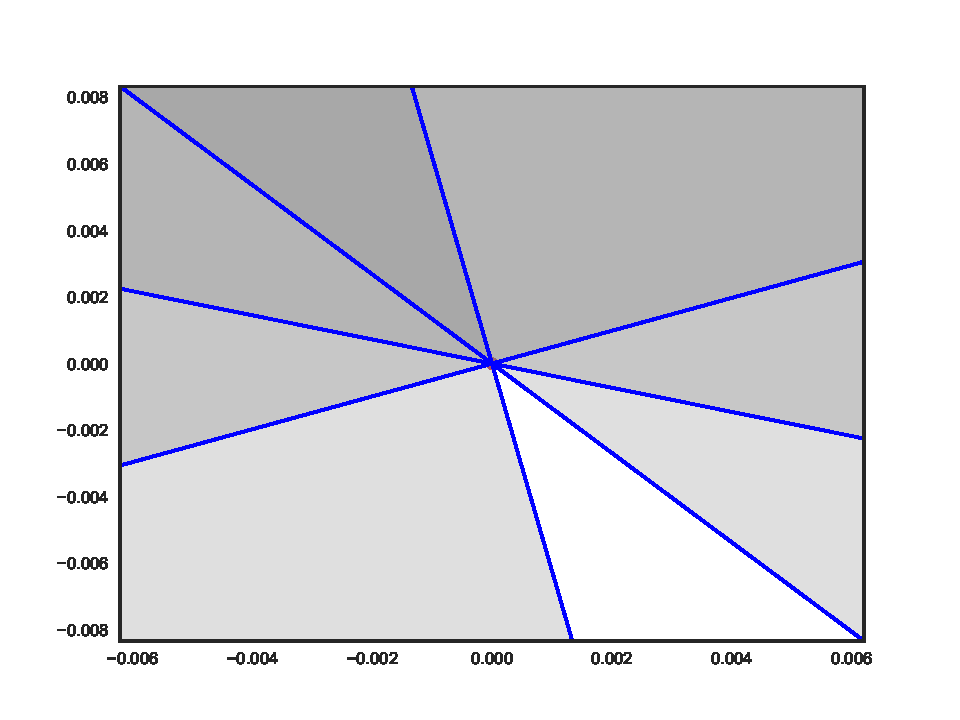
\includegraphics[width=\hsize]{img/toy/relu/conv2d_4-0.pdf}}
    %   \vskip1em
      \subcaptionbox{4th layer}{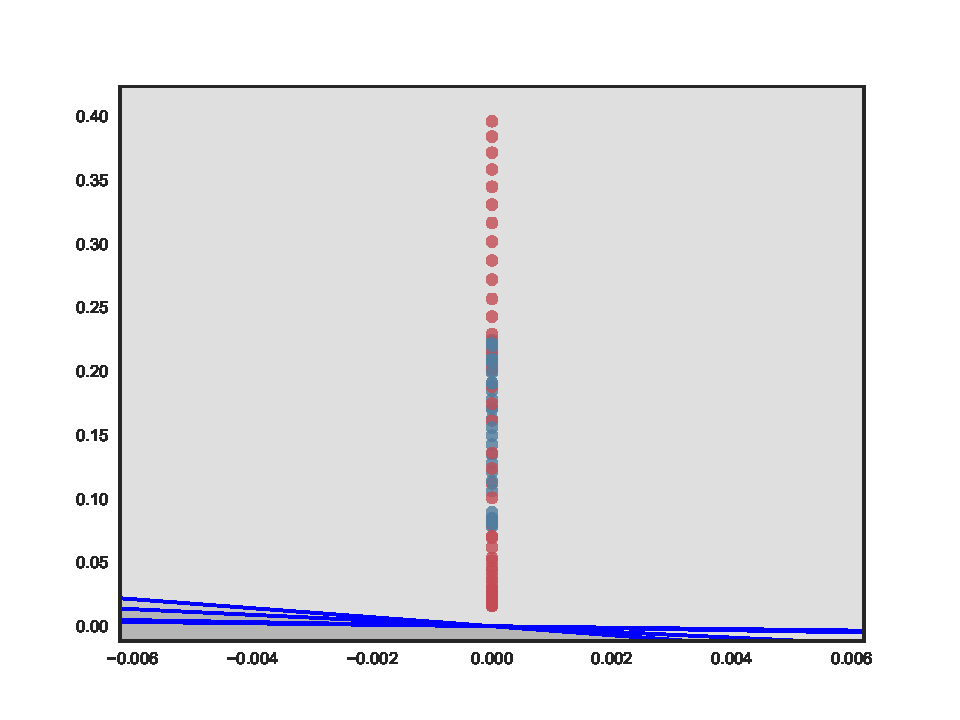
\includegraphics[width=\hsize]{img/toy/relu/conv2d_4-2.pdf}} 
    }
    % \hskip1em
    \parbox{.195\textwidth}{%
      \subcaptionbox{25th layer}{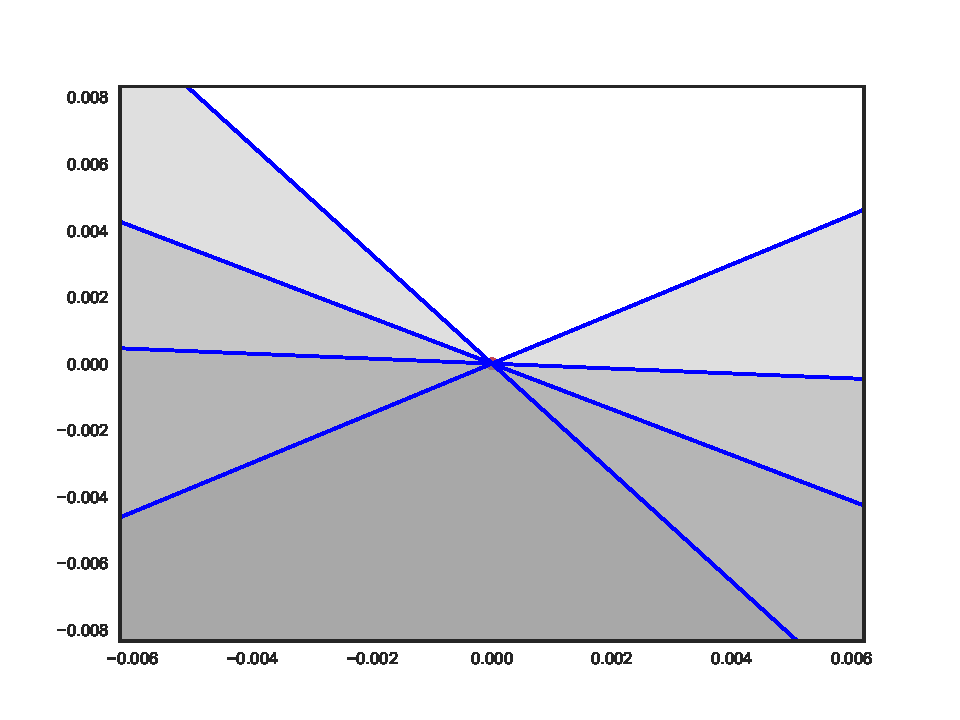
\includegraphics[width=\hsize]{img/toy/relu/conv2d_25-0.pdf}}
    %   \vskip1em
      \subcaptionbox{25th layer}{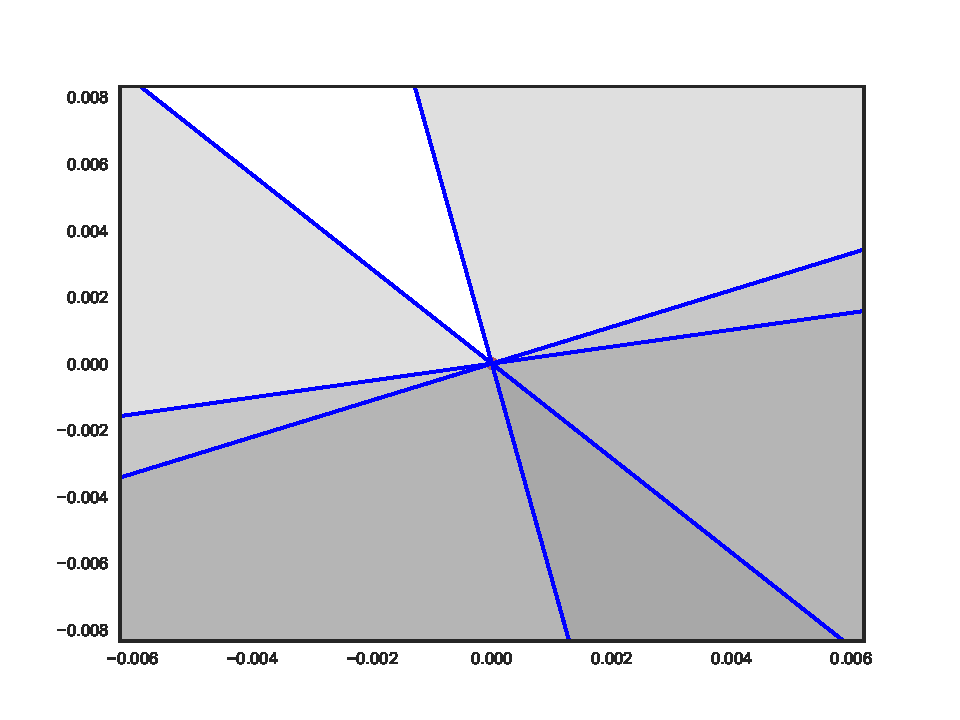
\includegraphics[width=\hsize]{img/toy/relu/conv2d_25-2.pdf}} 
    }
    % \hskip1em
    \parbox{.195\textwidth}{%
      \subcaptionbox{Feature layer}{\includegraphics[width=\hsize]{img/toy/relu/dense_1-0.pdf}}
    %   \vskip1em
      \subcaptionbox{Feature layer}{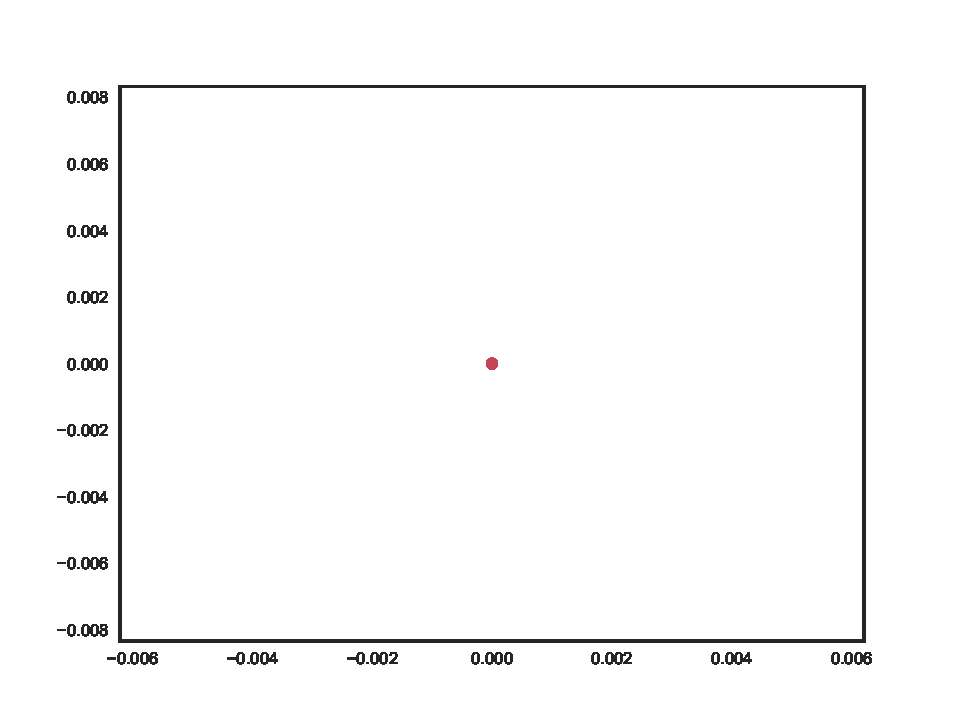
\includegraphics[width=\hsize]{img/toy/relu/dense_1-2.pdf}} 
    }
    % \hskip1em
    \parbox{.195\textwidth}{%
      \subcaptionbox{Output}{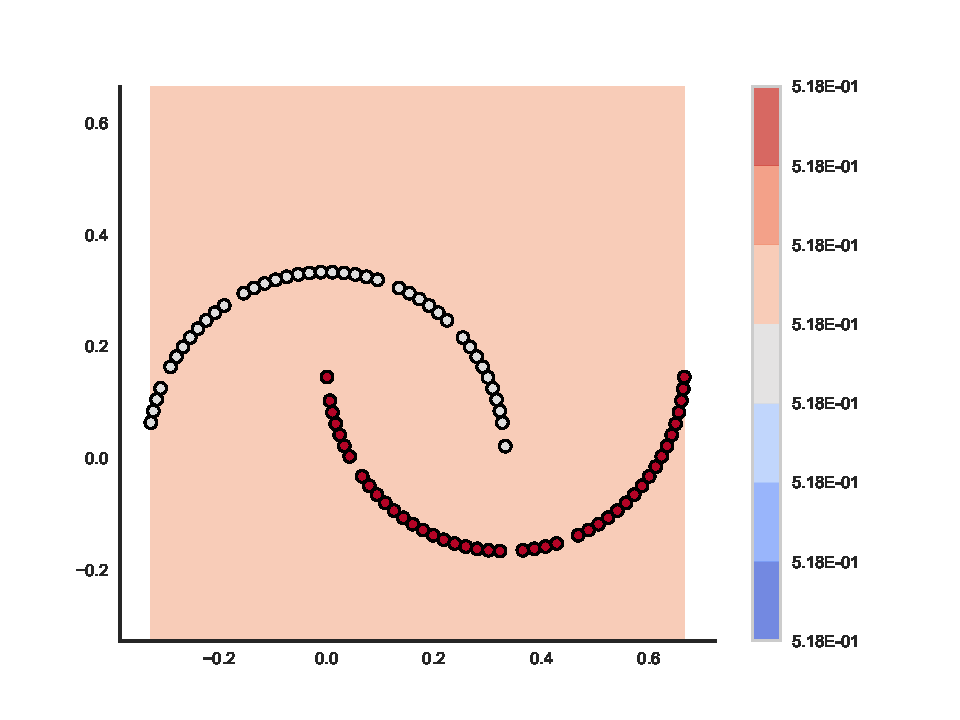
\includegraphics[width=\hsize]{img/toy/relu/output.pdf}}
    }
  }
  \caption{ReLU}
    \label{fig:moonsReLU}
\end{figure*}


Notice how the gradient has changed the separation performed by \ReLU in Figure \ref{fig:moonsReLU} at the input layer (a), but it fails to find a proper representation of use for the upper layers ((b), (c), (d)). The network shrinks the points to zero as they go across the network, to the point where in the 25th layer the entire dataset is in zero. This leads to the total failure to output anything useful (j), which in turn will make impossible to get gradient to overcome the situation. We say that the network is \emph{dead}. We argue that this is because the original placement of the hyperplanes in the layer by the initialization sends to zero a subset of the dataset at a time, so after a number of layers the entire dataset is zero. We undestand that with this all \emph{topological structure} of the network is lost. We relate this phenomena with the lack of smoothness over the transition across layers causing lack of \emph{intuitive} separation but taken to the extreme, described in \cite{hauserAsok}.

\begin{figure*}
  \centering
  \parbox{\textwidth}{
    \parbox{.195\textwidth}{%
      \subcaptionbox{Input layer}{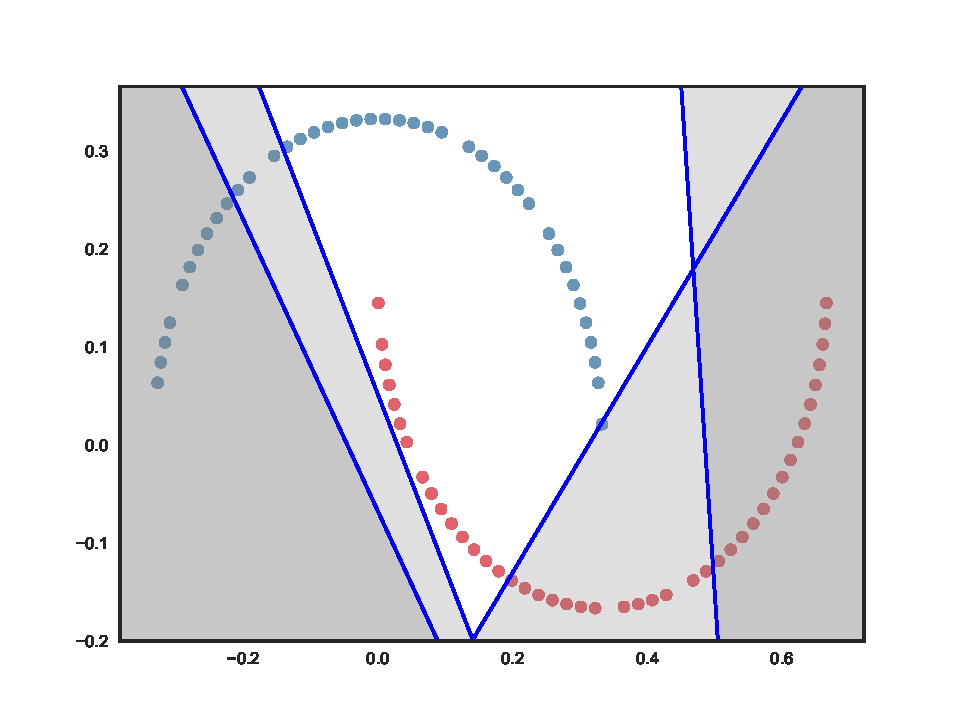
\includegraphics[width=\hsize]{img/toy/relu-bn/conv2d_1-0.pdf}}
    }
    % \hskip1em
    \parbox{.195\textwidth}{%
      \subcaptionbox{4th layer}{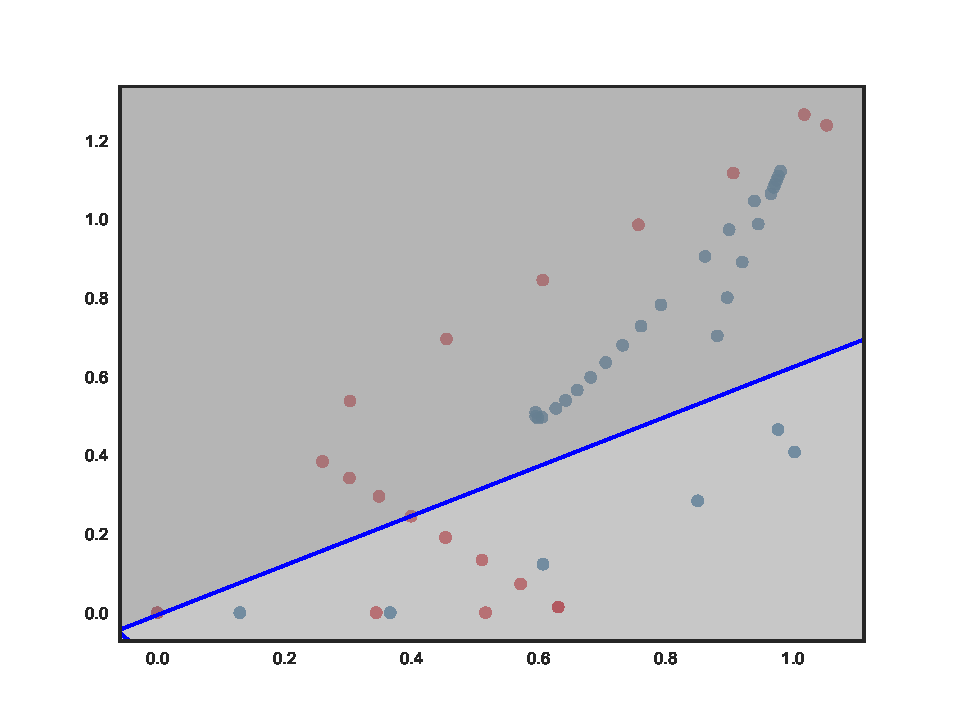
\includegraphics[width=\hsize]{img/toy/relu-bn/conv2d_4-0.pdf}}
    %   \vskip1em
      \subcaptionbox{4th layer}{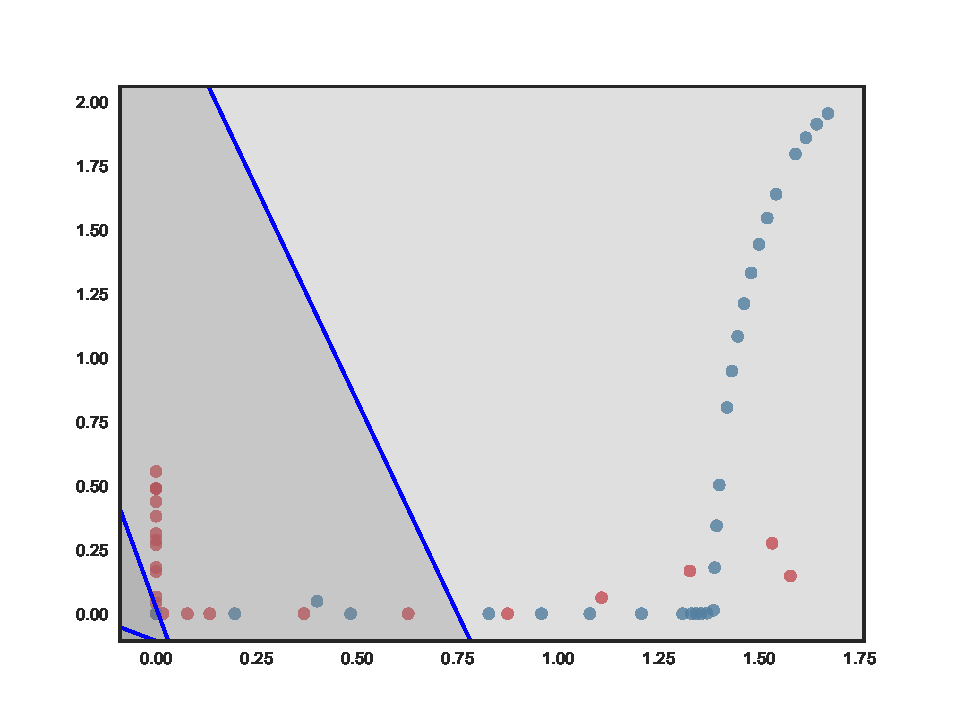
\includegraphics[width=\hsize]{img/toy/relu-bn/conv2d_4-2.pdf}}
    }
    % \hskip1em
    \parbox{.195\textwidth}{%
      \subcaptionbox{25th layer}{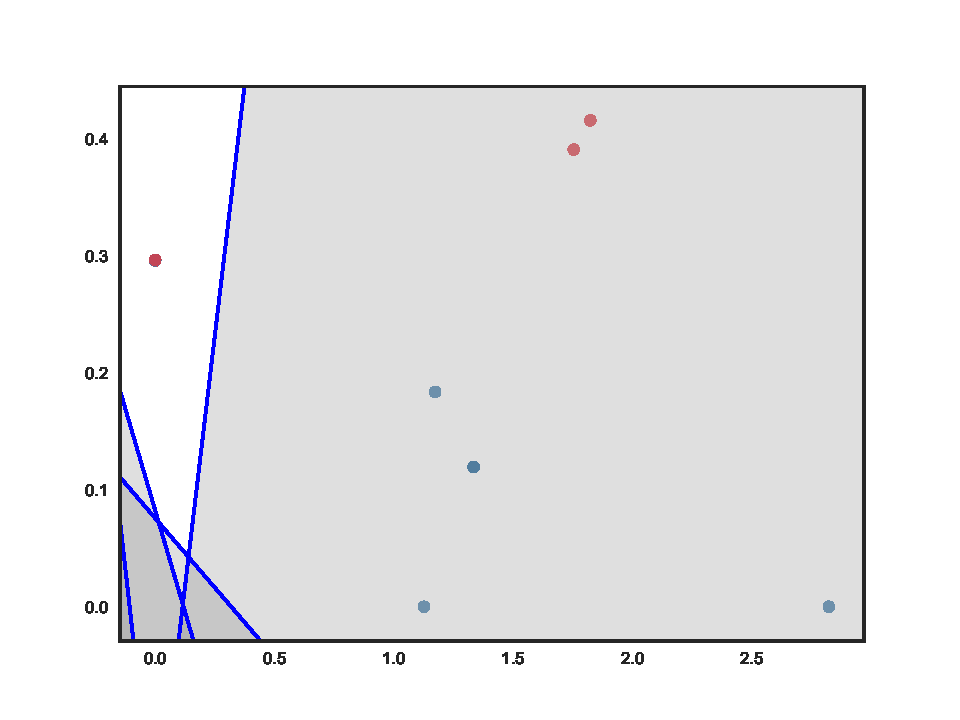
\includegraphics[width=\hsize]{img/toy/relu-bn/conv2d_25-0.pdf}}
    %   \vskip1em
      \subcaptionbox{25th layer}{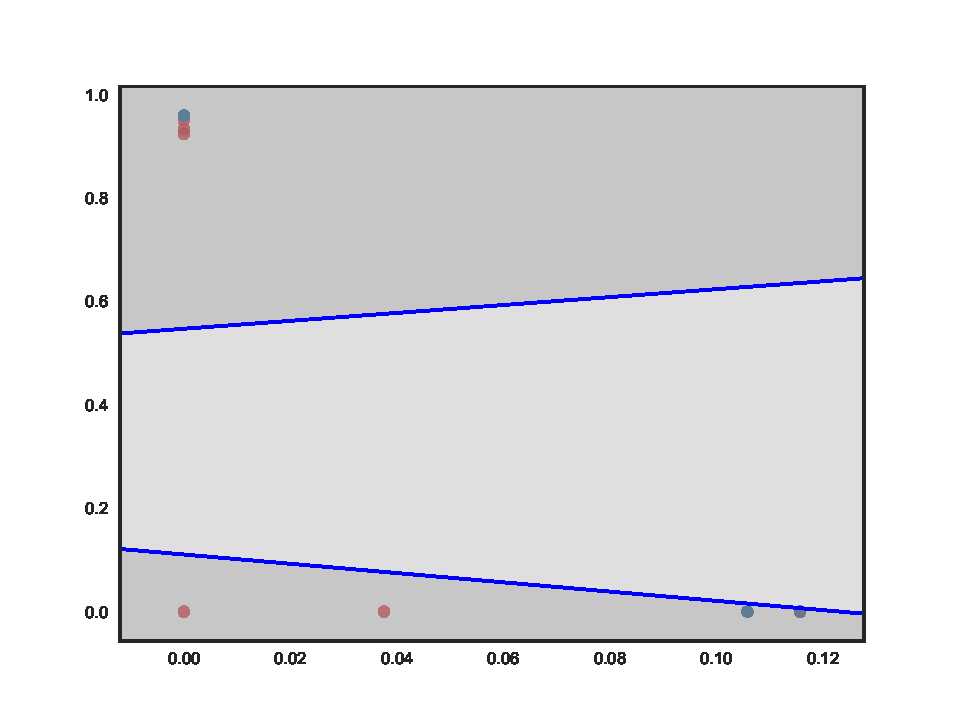
\includegraphics[width=\hsize]{img/toy/relu-bn/conv2d_25-2.pdf}} 
    }
    % \hskip1em
    \parbox{.195\textwidth}{%
      \subcaptionbox{}{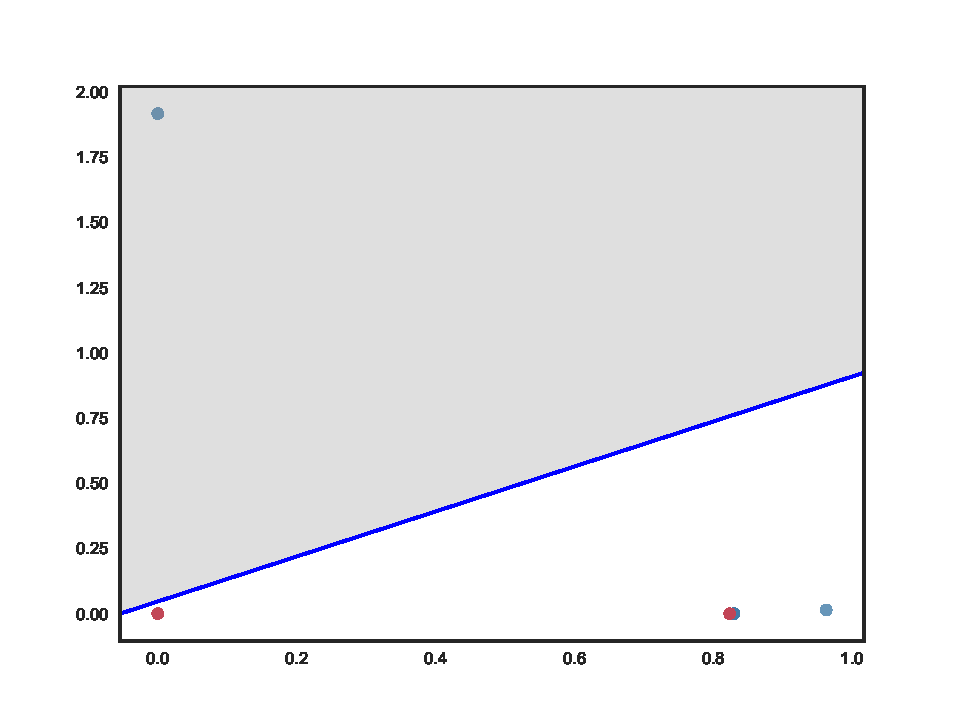
\includegraphics[width=\hsize]{img/toy/relu-bn/dense_1-0.pdf}}
    %   \vskip1em
      \subcaptionbox{}{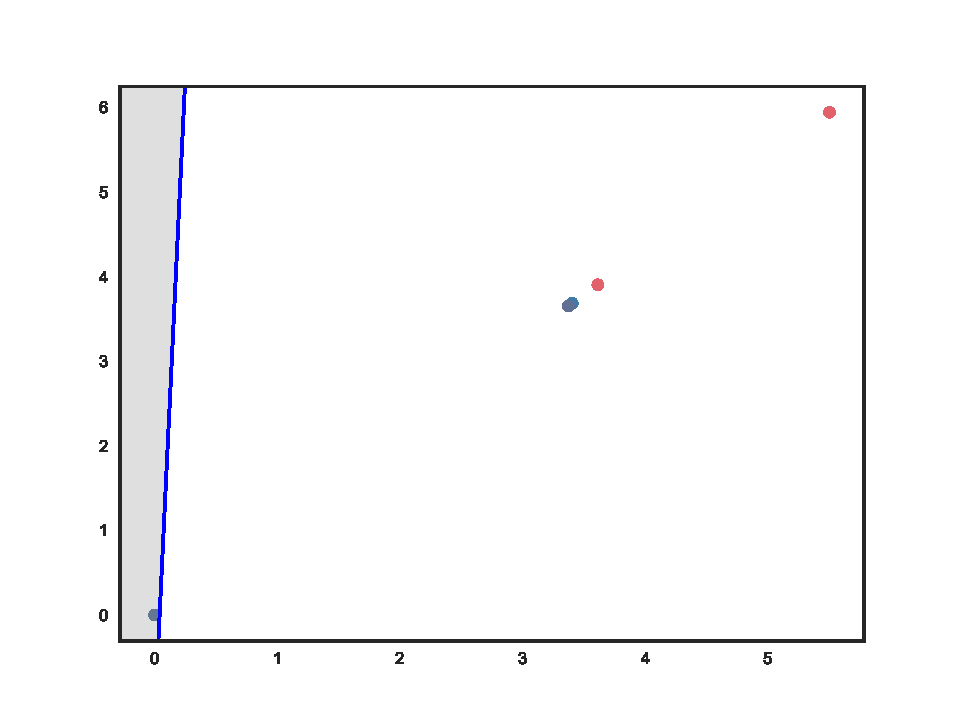
\includegraphics[width=\hsize]{img/toy/relu-bn/dense_1-2.pdf}} 
    }
    % \hskip1em
    \parbox{.195\textwidth}{%
      \subcaptionbox{Output}{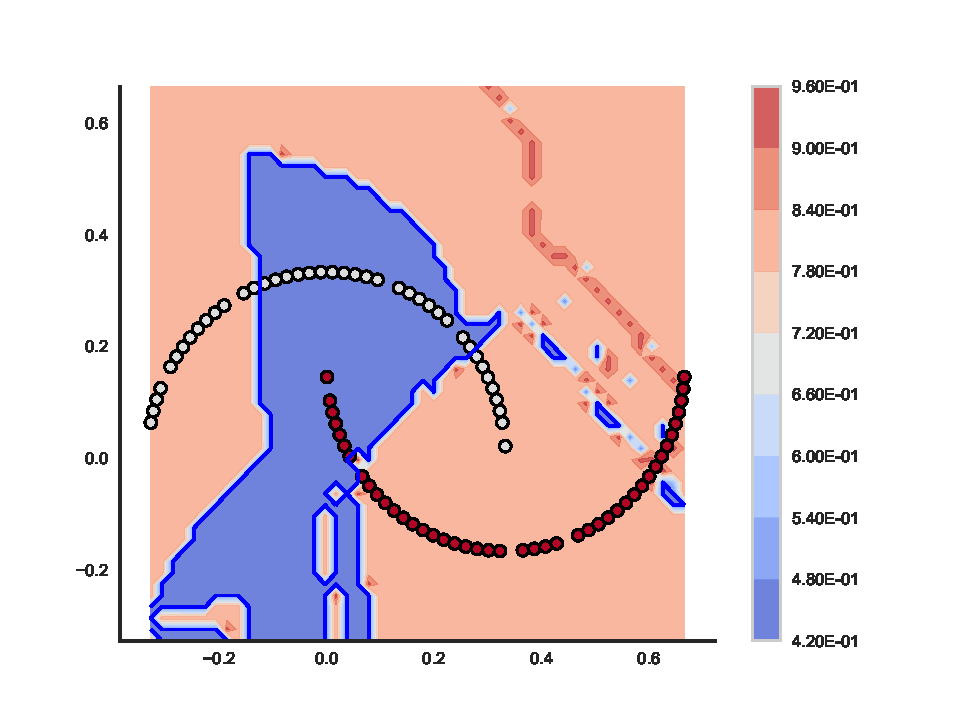
\includegraphics[width=\hsize]{img/toy/relu-bn/output.pdf}}
    }
  }
  \caption{\ReLUBN}
    \label{fig:moonsReLUBN}
\end{figure*}

\ReLUBN fares a bit better since it is able to pull the data out of zero, as we can see in the upper layers ((d), (e), (f), (g)), yet it is still unable to preserve the \emph{topological structure} like \ReLU, which ultimately leads to \emph{topologically mixing} \cite{hirsch2012differential}, in a fashion similar to the \emph{baker's map}. This generates very strange outputs which we can see in (h) whose gradients fail again to provide hints to the lower layers to fix the topological structure of the network. 

\begin{figure*}
  \centering
  \parbox{\textwidth}{
    \parbox{.195\textwidth}{%
      \subcaptionbox{Input layer}{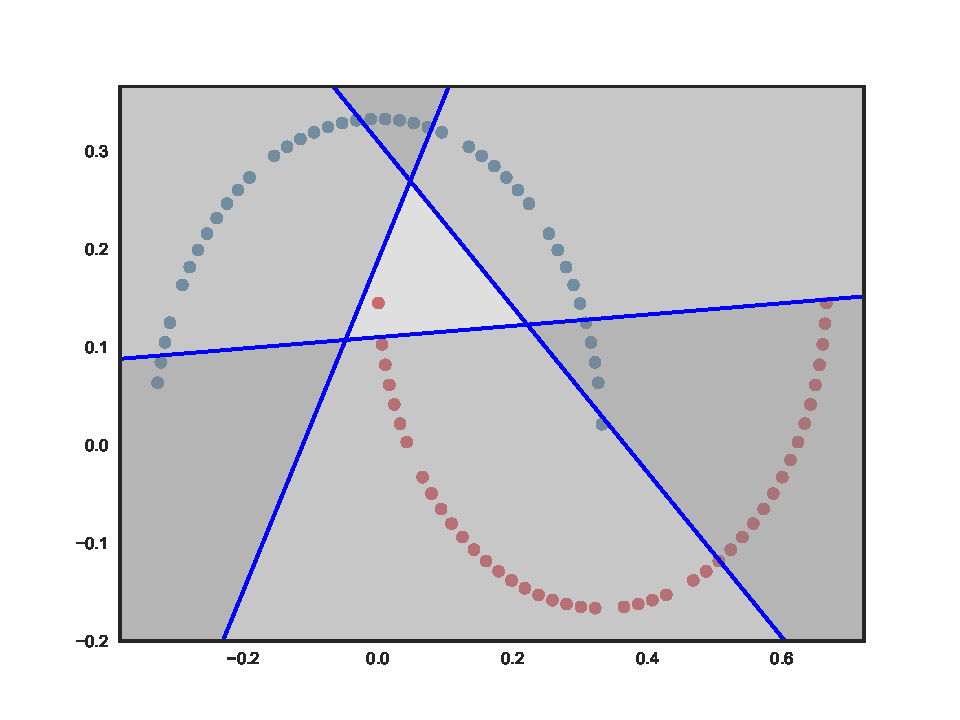
\includegraphics[width=\hsize]{img/toy/layerwise/conv2d_1-0.pdf}}
    }
    % \hskip1em
    \parbox{.195\textwidth}{%
      \subcaptionbox{4th layer}{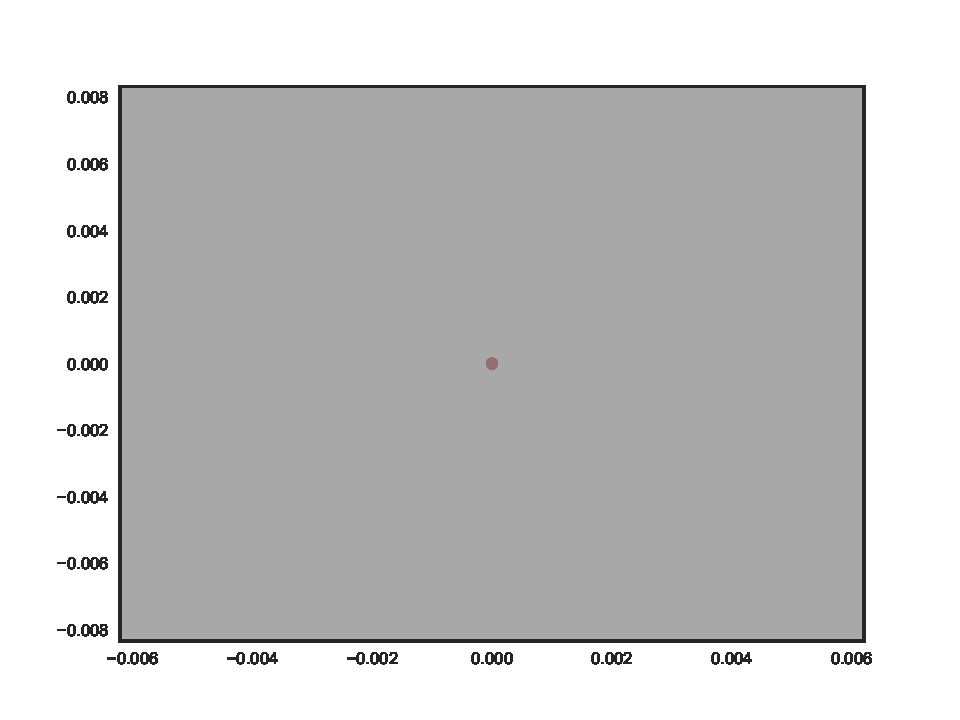
\includegraphics[width=\hsize]{img/toy/layerwise/conv2d_4-0.pdf}}
    %   \vskip1em
      \subcaptionbox{4th layer}{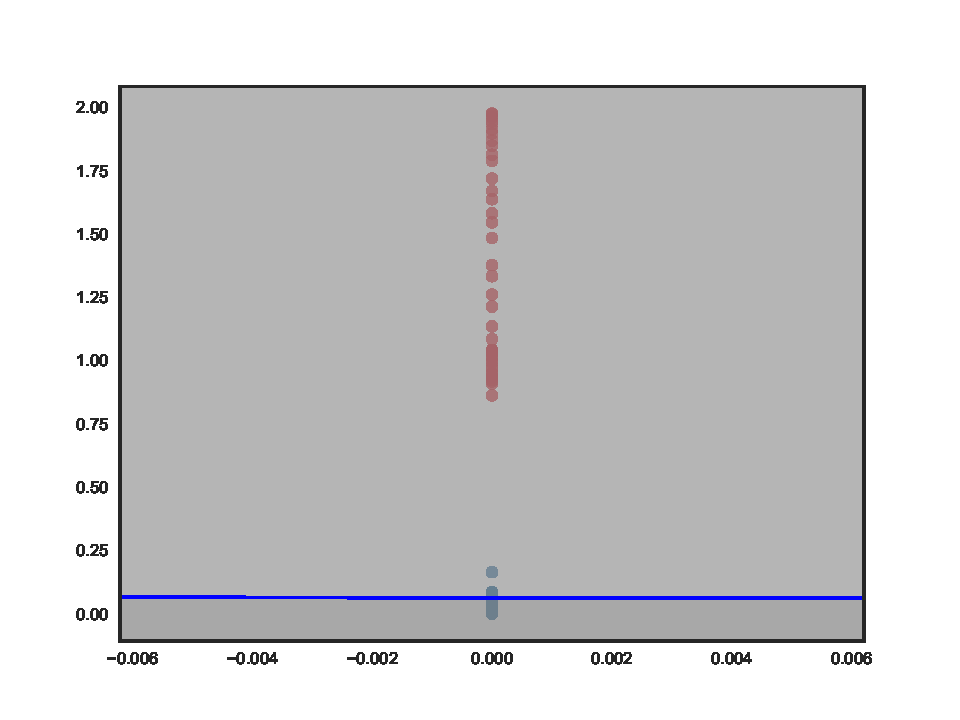
\includegraphics[width=\hsize]{img/toy/layerwise/conv2d_4-2.pdf}} 
    }
    % \hskip1em
    \parbox{.195\textwidth}{%
      \subcaptionbox{25th layer}{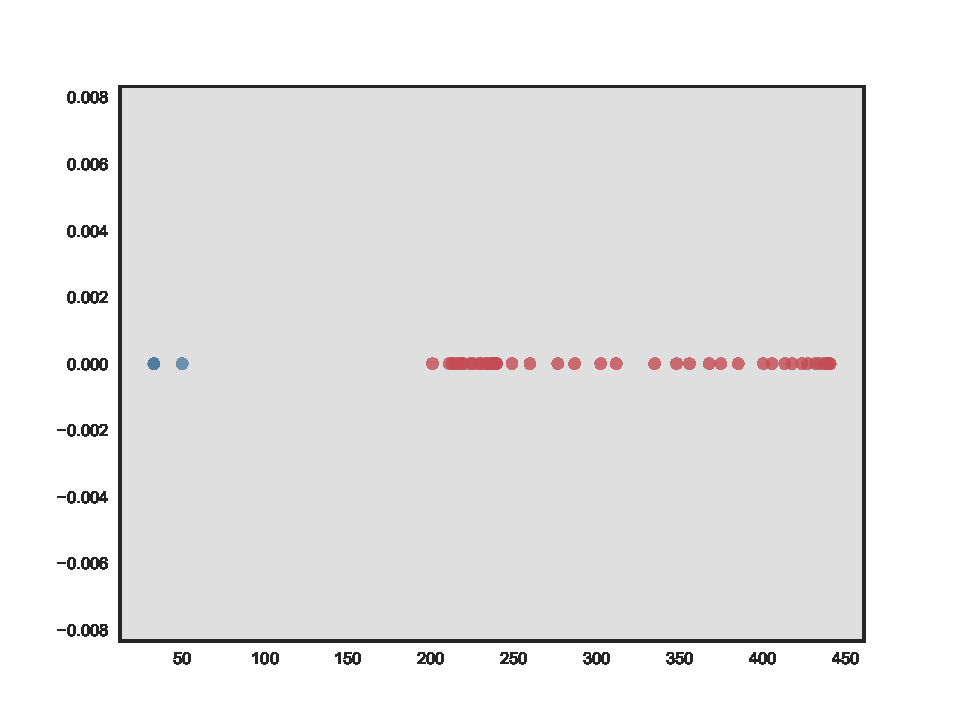
\includegraphics[width=\hsize]{img/toy/layerwise/conv2d_25-0.pdf}}
    %   \vskip1em
      \subcaptionbox{25th layer}{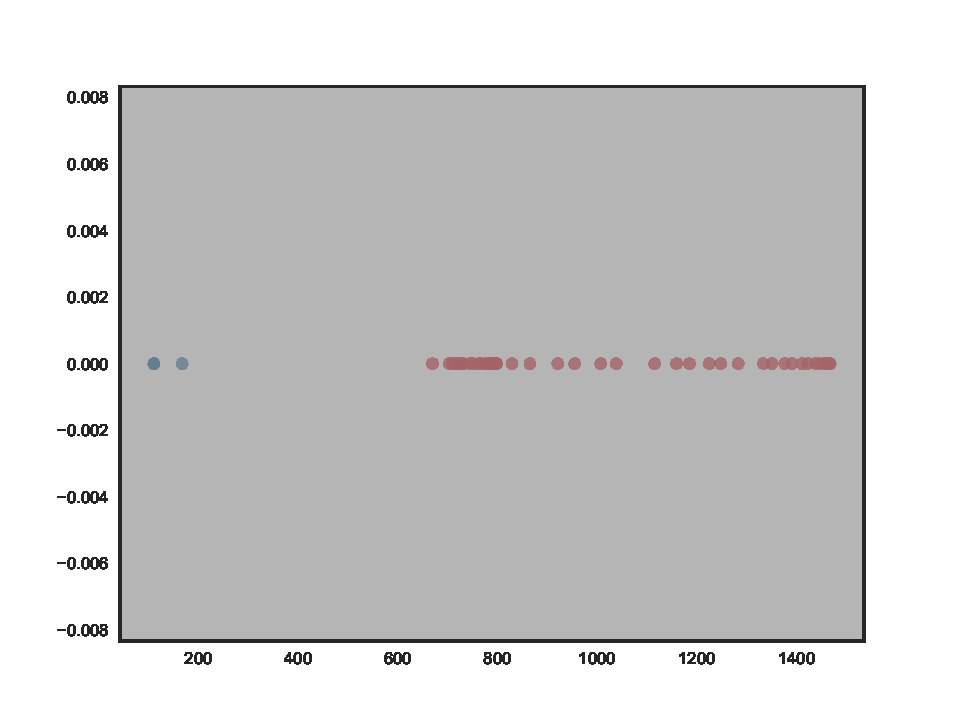
\includegraphics[width=\hsize]{img/toy/layerwise/conv2d_25-2.pdf}} 
    }
    % \hskip1em
    \parbox{.195\textwidth}{%
      \subcaptionbox{Feature layer}{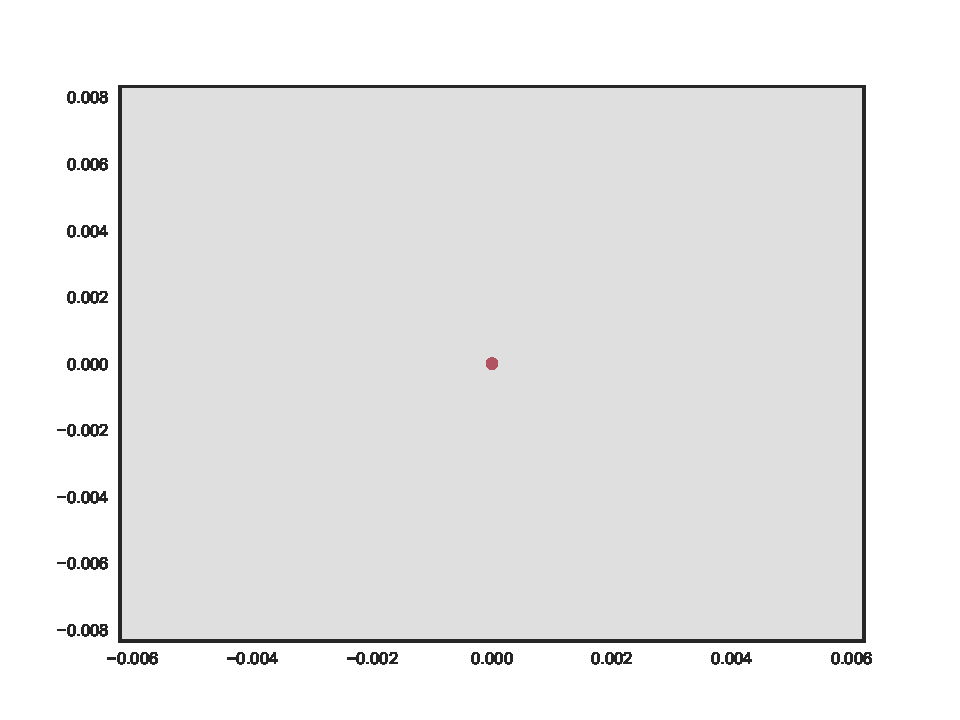
\includegraphics[width=\hsize]{img/toy/layerwise/dense_1-0.pdf}}
    %   \vskip1em
      \subcaptionbox{Feature layer}{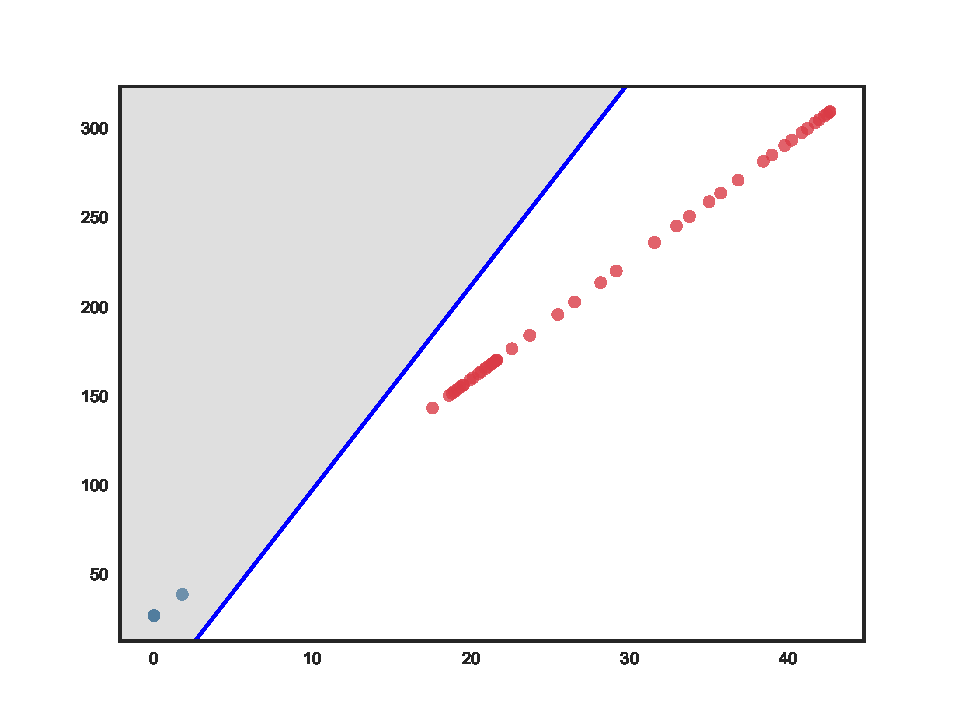
\includegraphics[width=\hsize]{img/toy/layerwise/dense_1-2.pdf}} 
    }
    % \hskip1em
    \parbox{.195\textwidth}{%
      \subcaptionbox{Output}{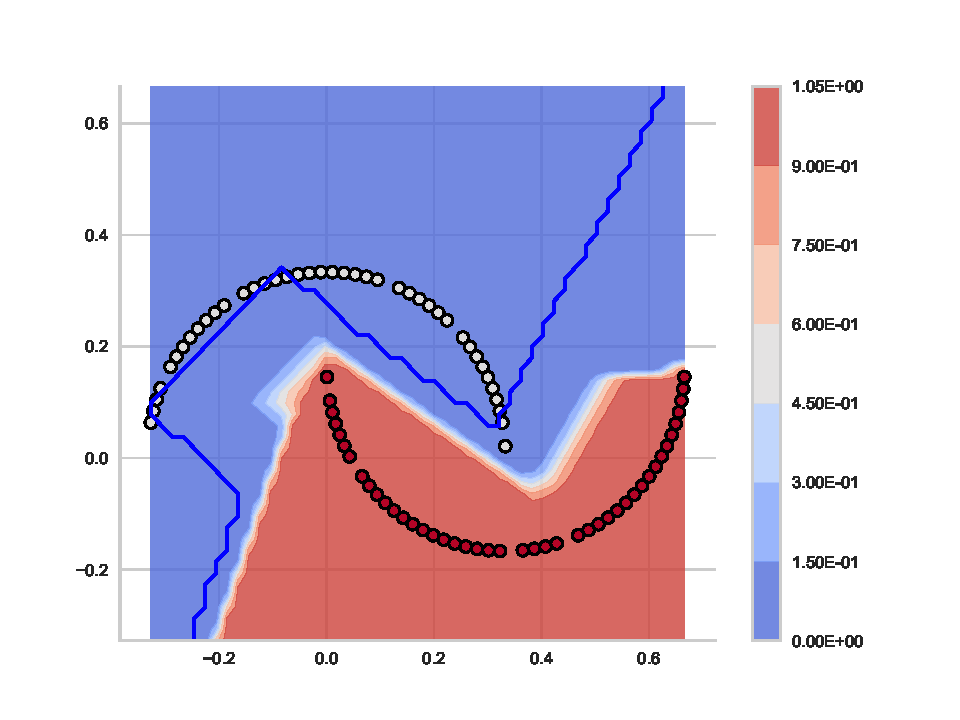
\includegraphics[width=\hsize]{img/toy/layerwise/output.pdf}}
    }
  }
    \caption{\SepLayer}
    \label{fig:moonsLayerwise}
\end{figure*}


In the other hand, our relaxed version of our proposal \SepLayer, see Figure \ref{fig:moonsLayerwise}, is able to solve the problem (h). We find how is able to propagate the information needed for the lower layers to perform the separation, so we can see at (k) how the separating planes are much better placed, so by the bottom layers (c) the problem is already solved and the rest of layers simply forward upwards ((d), (e)). Since our formulation \SepLayer is a relaxed version of \SepUnit we allow are redundant and dead units. Notice how the entire space is colored in different shades of gray, showing how at (d) least one unit is effectively operating in linear mode, thus proving how in certain situations affine units might be useful by forwarding information into deeper layers. 

\begin{figure*}
  \centering
     % Unitwise
  \parbox{\textwidth}{
    \parbox{.195\textwidth}{%
      \subcaptionbox{Input layer}{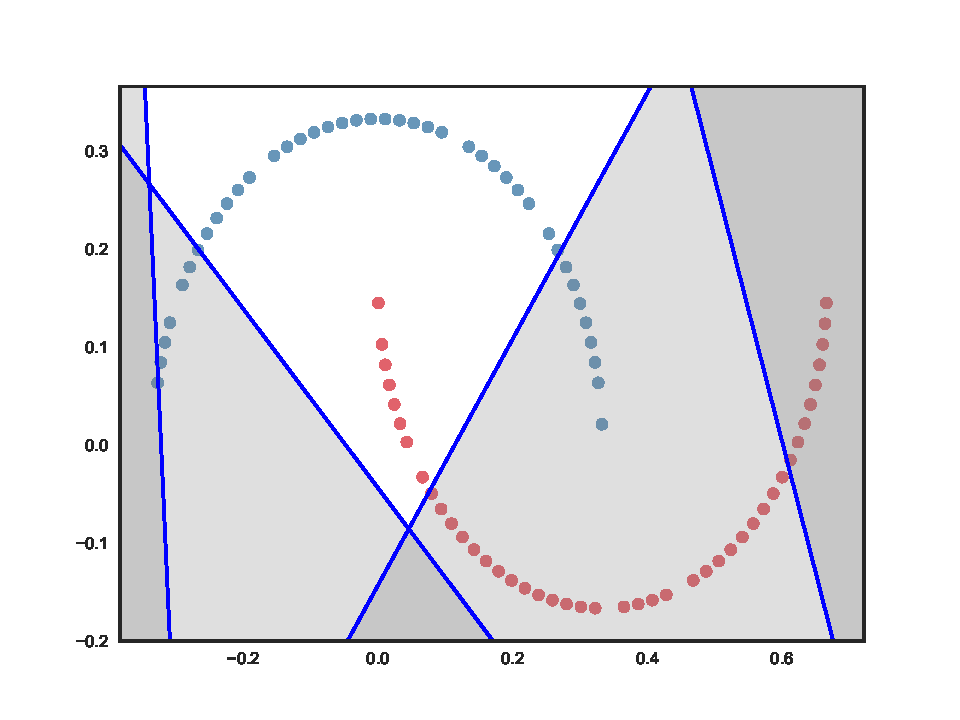
\includegraphics[width=\hsize]{img/toy/unitwise/conv2d_1-0.pdf}}
    }
    % \hskip1em
    \parbox{.195\textwidth}{%
      \subcaptionbox{4th layer}{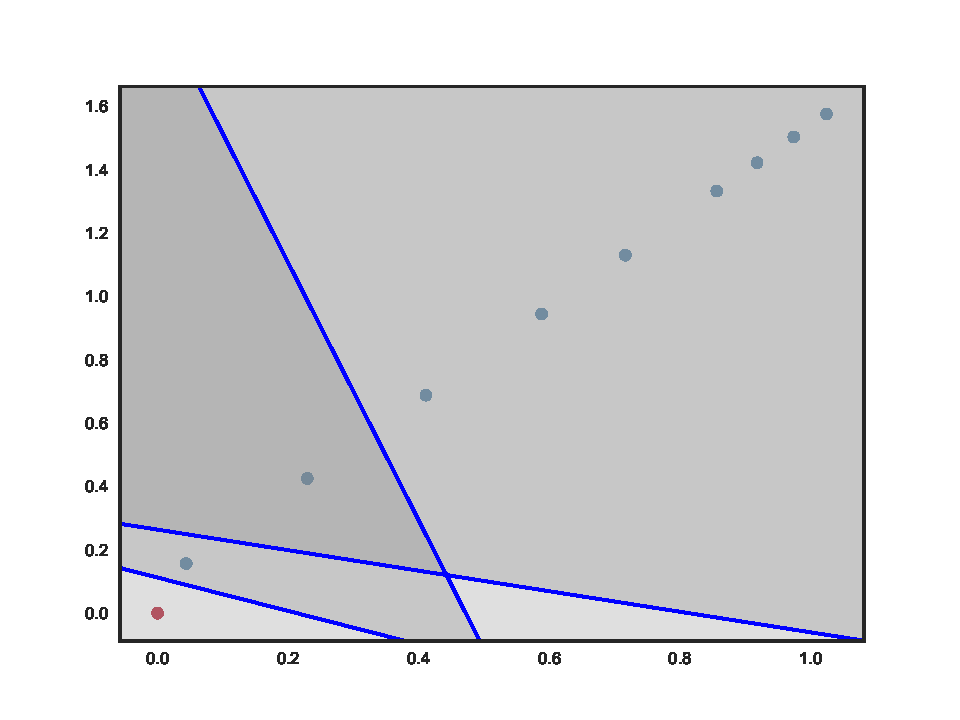
\includegraphics[width=\hsize]{img/toy/unitwise/conv2d_4-0.pdf}}
    %   \vskip1em
      \subcaptionbox{4th layer}{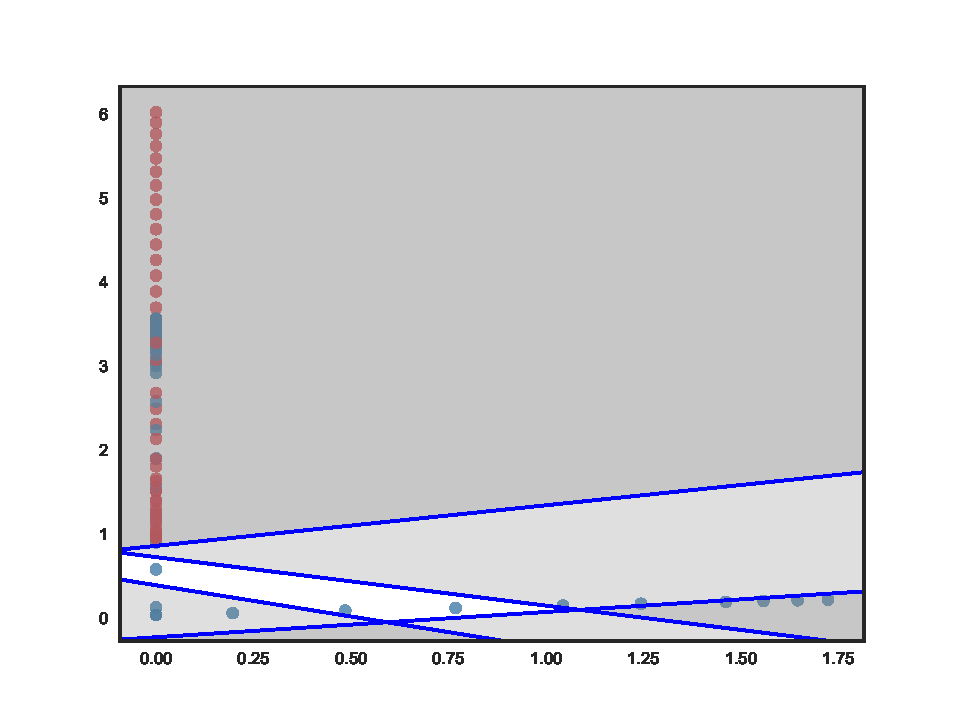
\includegraphics[width=\hsize]{img/toy/unitwise/conv2d_4-2.pdf}} 
    }
    % \hskip1em
    \parbox{.195\textwidth}{%
      \subcaptionbox{25th layer}{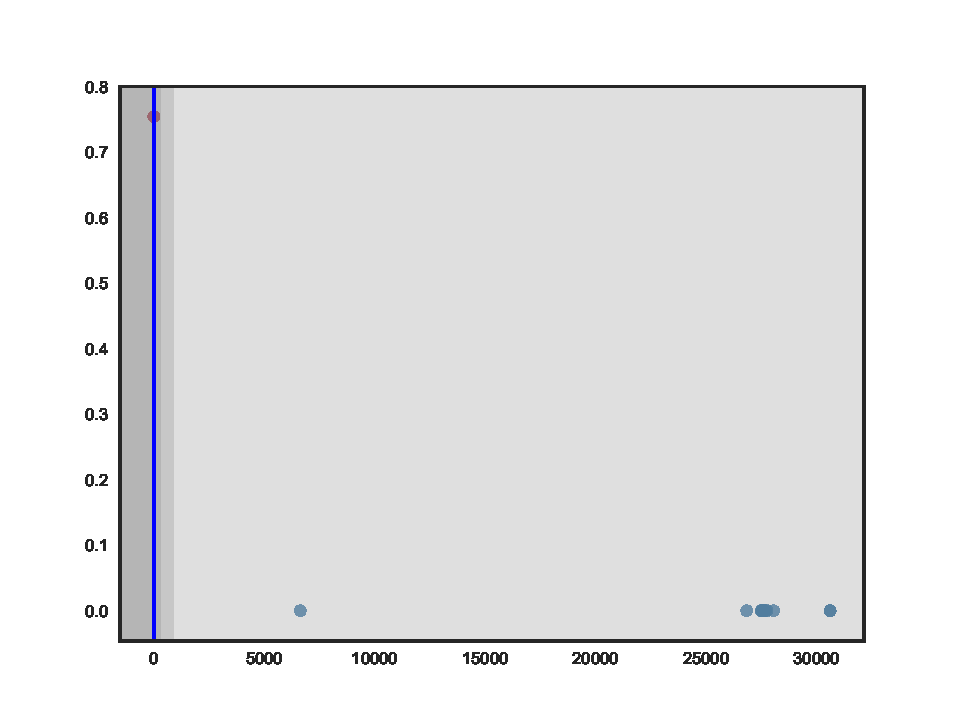
\includegraphics[width=\hsize]{img/toy/unitwise/conv2d_25-0.pdf}}
    %   \vskip1em
      \subcaptionbox{25th layer}{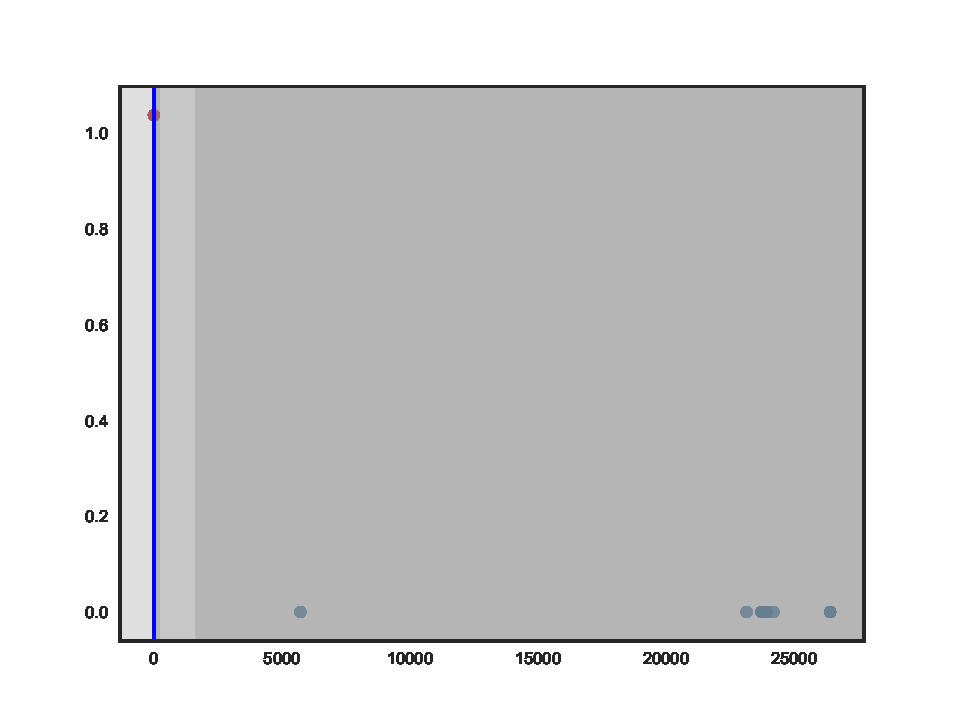
\includegraphics[width=\hsize]{img/toy/unitwise/conv2d_25-2.pdf}} 
    }
    % \hskip1em
    \parbox{.195\textwidth}{%
      \subcaptionbox{Feature layer}{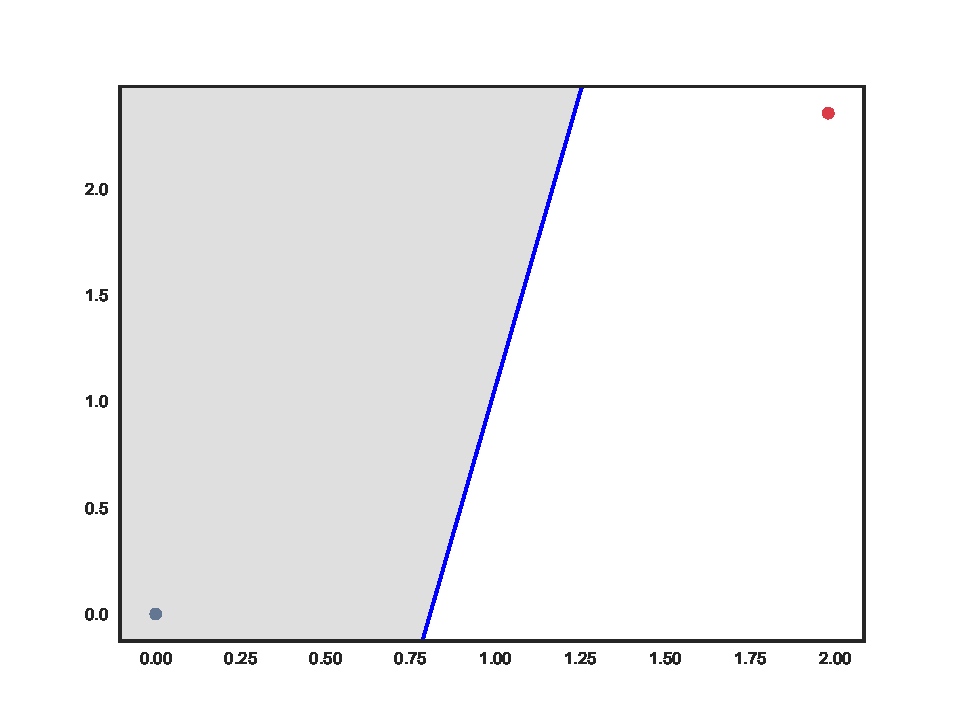
\includegraphics[width=\hsize]{img/toy/unitwise/dense_1-0.pdf}}
    %   \vskip1em
      \subcaptionbox{Feature layer}{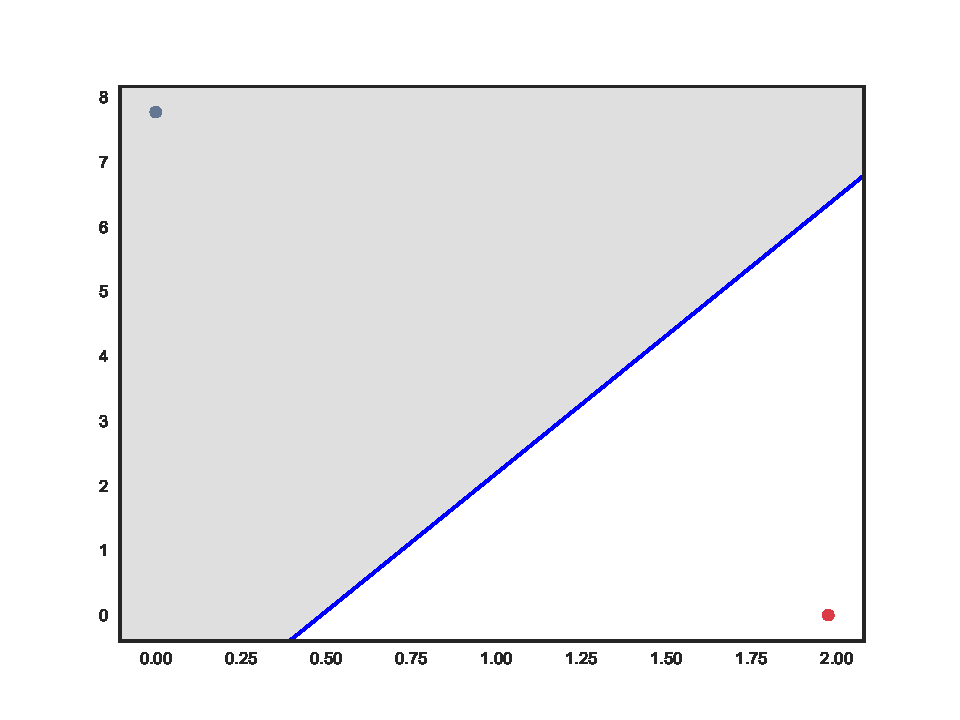
\includegraphics[width=\hsize]{img/toy/unitwise/dense_1-2.pdf}} 
    }
    % \hskip1em
    \parbox{.195\textwidth}{%
      \subcaptionbox{Output}{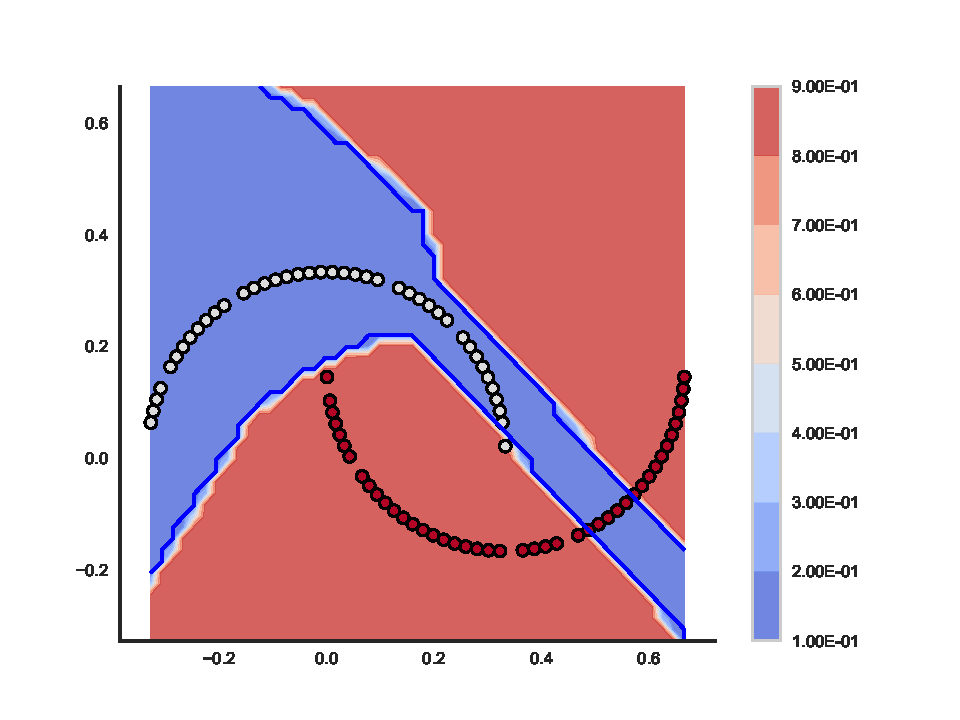
\includegraphics[width=\hsize]{img/toy/unitwise/output.pdf}}
    }
  }
  \caption{\SepUnit}
    \label{fig:moonsUnitwise}
\end{figure*}


Figure \ref{fig:moonsUnitwise} shows our restricted version \SepUnit, which forces all the units of the network to separate but does not consider activation with regard to the points. Because this, solutions like activating all the units of the layer for a single point and sending the rest to zero are still valid, as we explained in \ref{eq:unitFail}. Therefore, we expect it to fail. However, the network still converges to a close to optimal solution. Notice how the feature layer \ref{fig:moonsUnitwise}(f,g) is much more polarized than \SepLayer \ref{fig:moonsLayerwise}(f,g), similar to \ReLUBN \ref{fig:moonsReLUBN}(f,g), although the solution is much better and the representation at layer 25 (d,e) is richer. However, this solution is transitory and the training breaks after some epochs. Further research is thus required in this regard.

\begin{figure*}
  \centering
  %Pointwise
  \parbox{\textwidth}{
    \parbox{.195\textwidth}{%
      \subcaptionbox{Input layer}{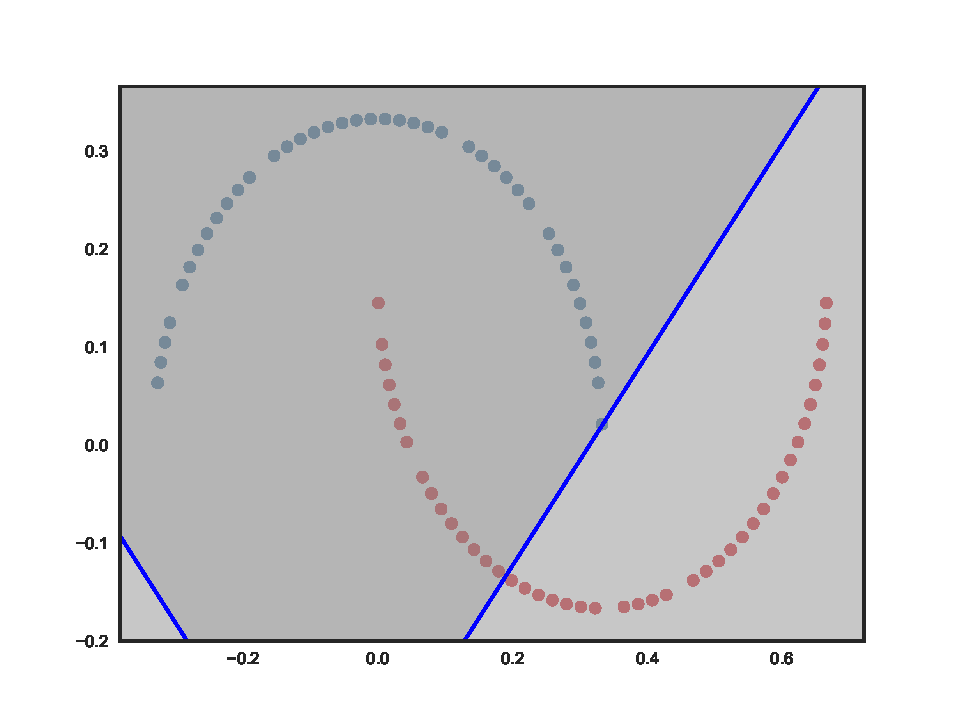
\includegraphics[width=\hsize]{img/toy/pointwise/conv2d_1-0.pdf}}
    }
    % \hskip1em
    \parbox{.195\textwidth}{%
      \subcaptionbox{4th layer}{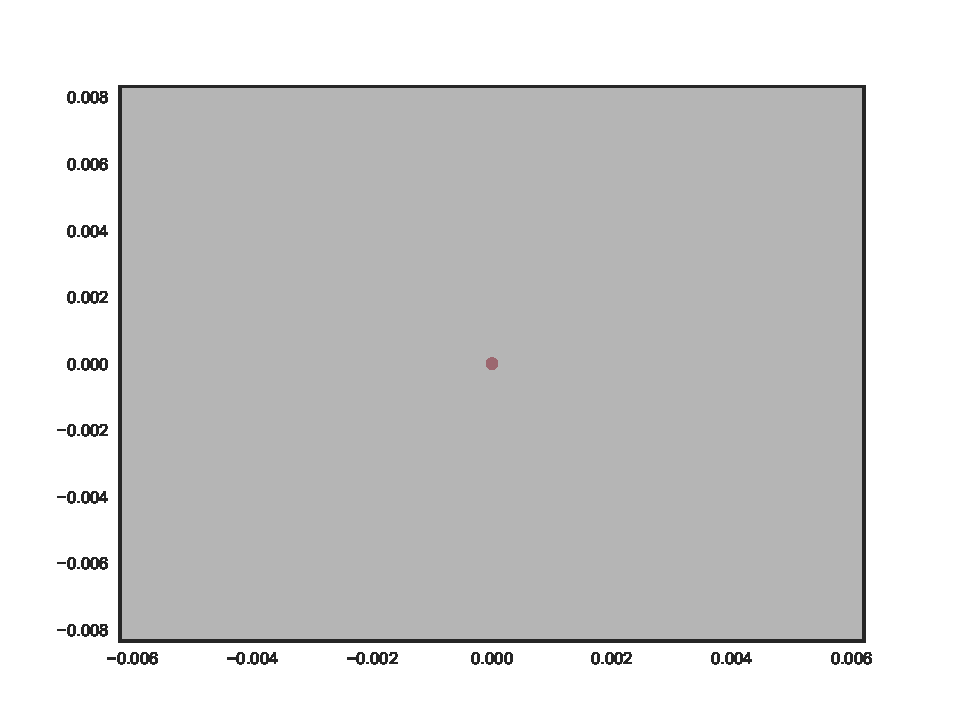
\includegraphics[width=\hsize]{img/toy/pointwise/conv2d_4-0.pdf}}
    %   \vskip1em
      \subcaptionbox{4th layer}{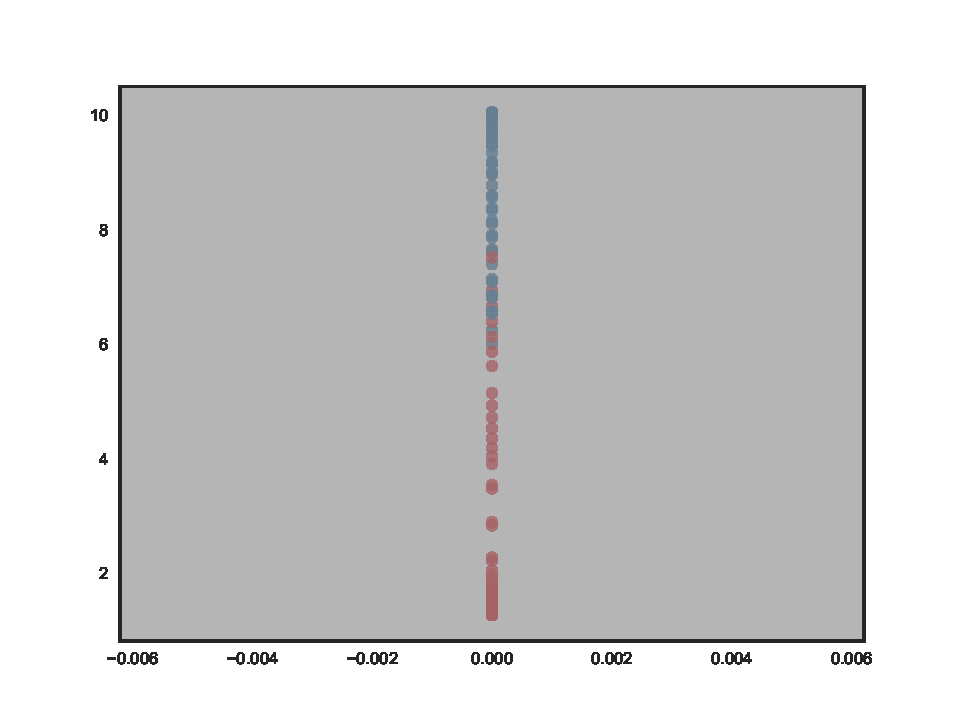
\includegraphics[width=\hsize]{img/toy/pointwise/conv2d_4-2.pdf}} 
    }
    % \hskip1em
    \parbox{.195\textwidth}{%
      \subcaptionbox{25th layer}{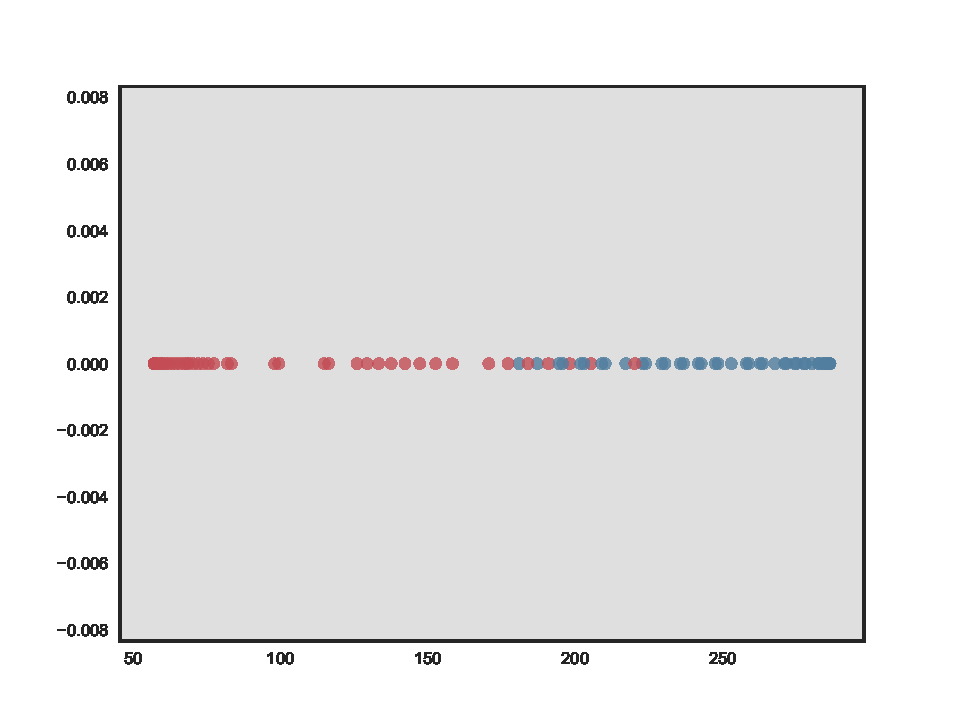
\includegraphics[width=\hsize]{img/toy/pointwise/conv2d_25-0.pdf}}
    %   \vskip1em
      \subcaptionbox{25th layer}{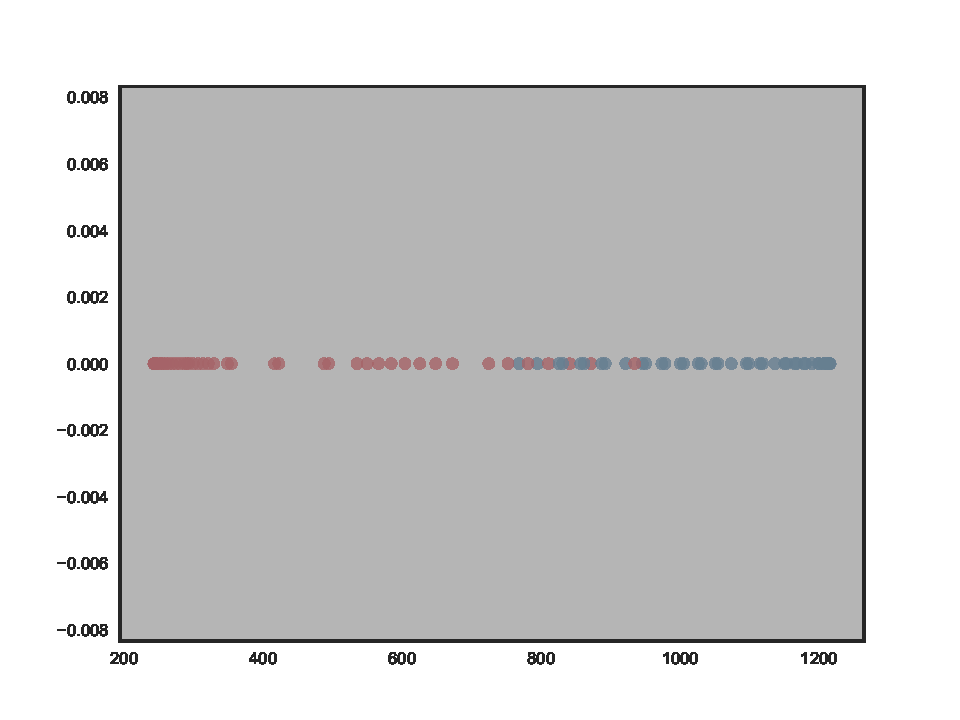
\includegraphics[width=\hsize]{img/toy/pointwise/conv2d_25-2.pdf}} 
    }
    % \hskip1em
    \parbox{.195\textwidth}{%
      \subcaptionbox{}{\includegraphics[width=\hsize]{img/toy/pointwise/dense_1-0.pdf}}
    %   \vskip1em
      \subcaptionbox{}{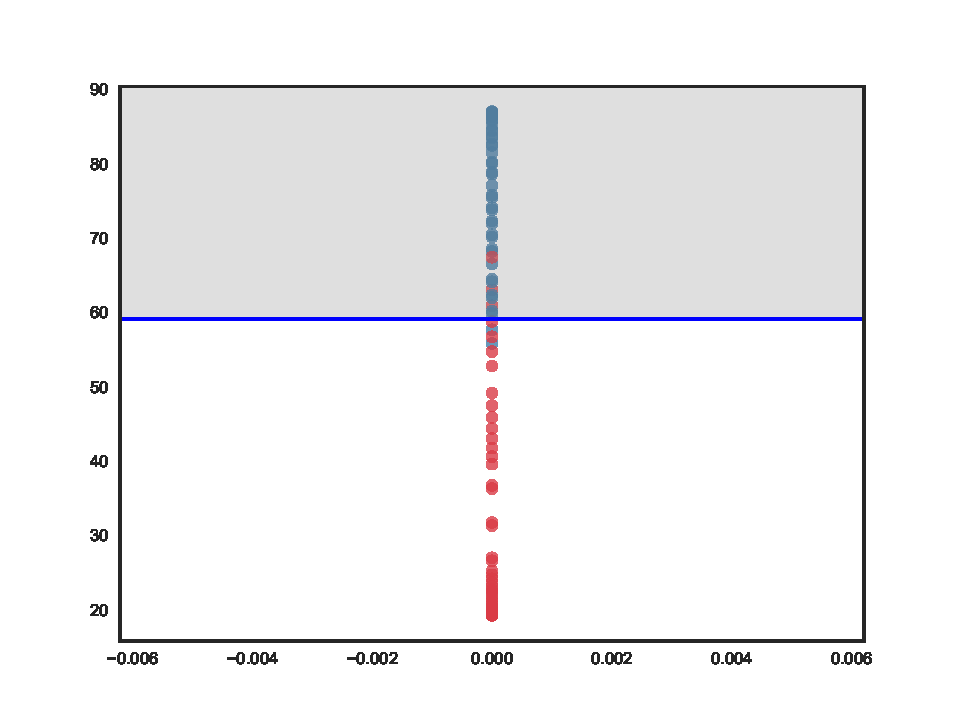
\includegraphics[width=\hsize]{img/toy/pointwise/dense_1-2.pdf}} 
    }
    % \hskip1em
    \parbox{.195\textwidth}{%
      \subcaptionbox{Output}{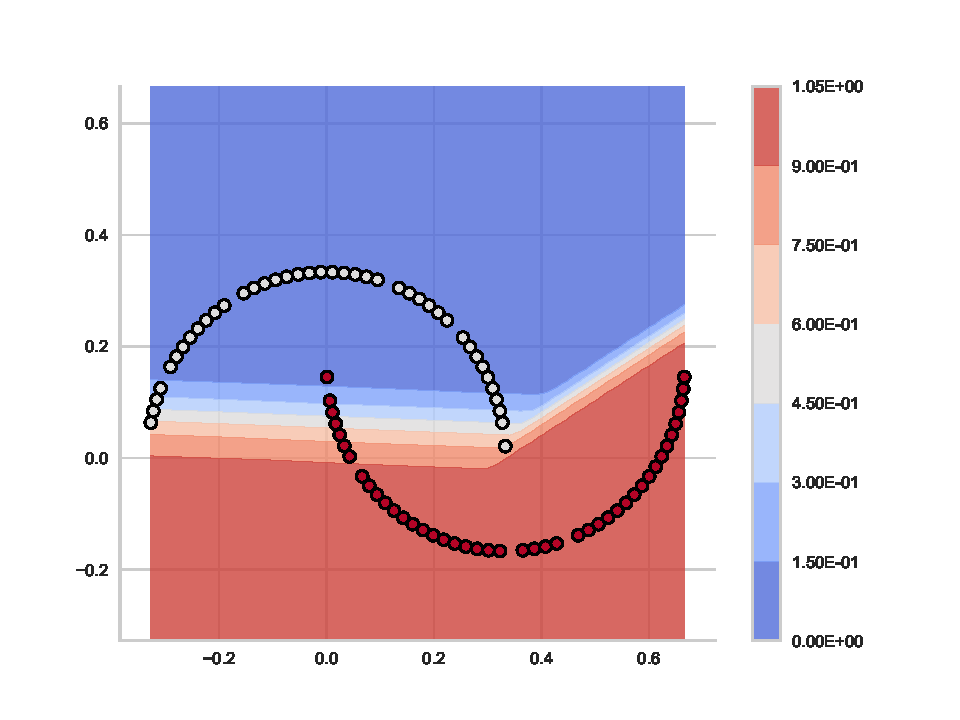
\includegraphics[width=\hsize]{img/toy/pointwise/output.pdf}}
    }
  }
  \caption{\SepPoint}
    \label{fig:moonsPointwise}
\end{figure*}

The constraint \SepPoint is shown at Figure \ref{fig:moonsPointwise}. We see how it effectively propagates the data \emph{topological structure} up to the output of the network ((e), (d), (f), (g)), but as the only requirement that for each point at least one unit is activated and another not this can be fulfilled with an affine unit, so the solution remains almost linear (h). 

\begin{figure*}
  \centering
   \parbox{\textwidth}{
    \parbox{.195\textwidth}{%
      \subcaptionbox{Input layer}{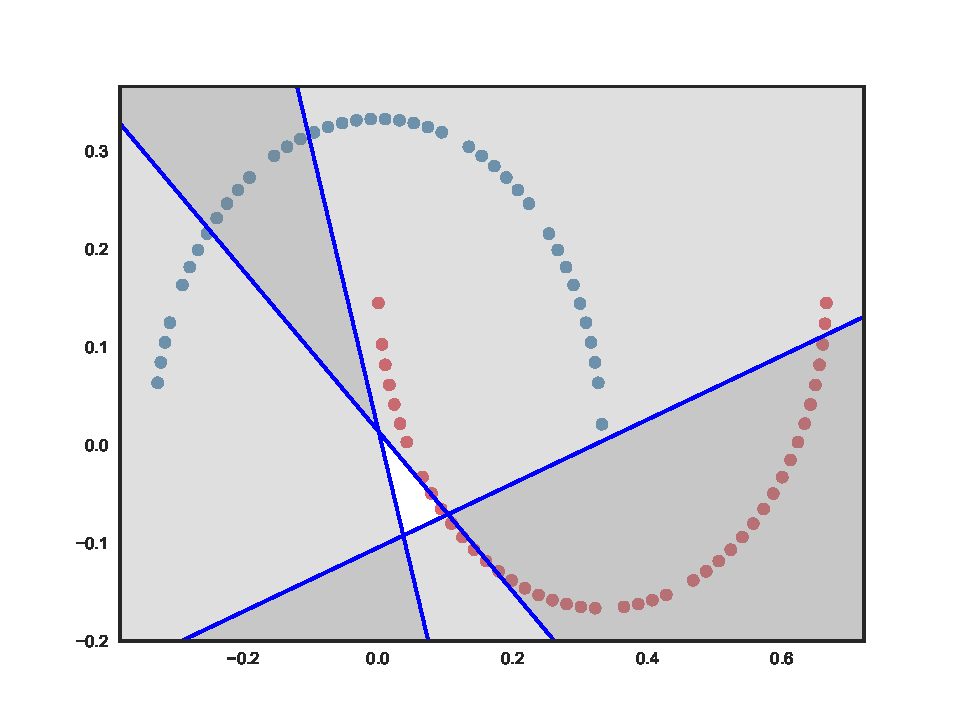
\includegraphics[width=\hsize]{img/toy/unitpointwise/conv2d_1-0.pdf}}
    }
    % \hskip1em
    \parbox{.195\textwidth}{%
      \subcaptionbox{4th layer}{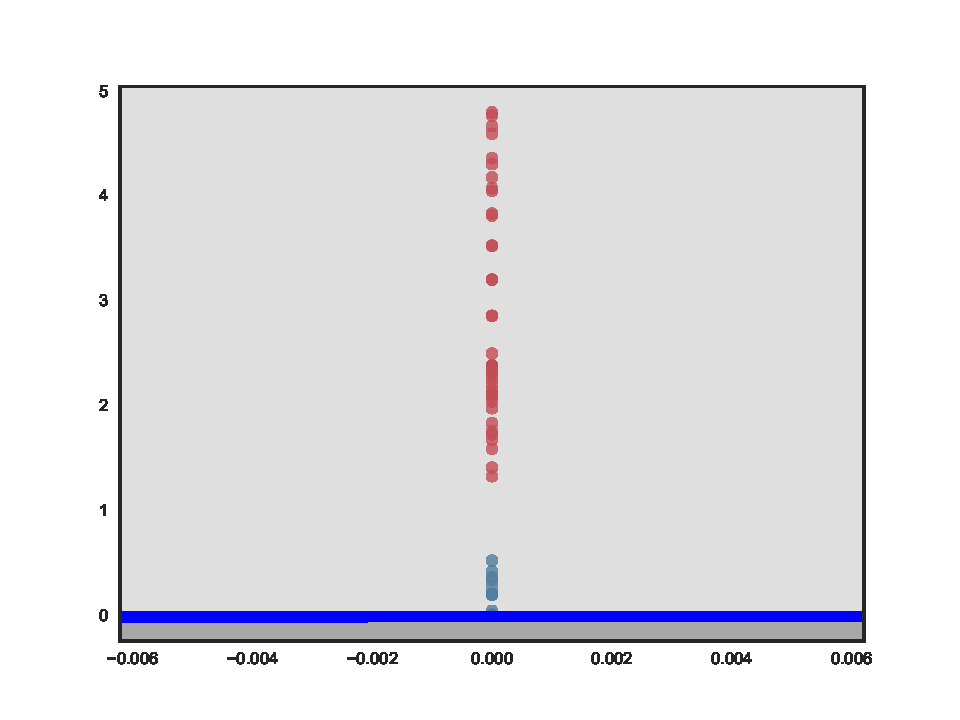
\includegraphics[width=\hsize]{img/toy/unitpointwise/conv2d_4-0.pdf}}
    %   \vskip1em
      \subcaptionbox{4th layer}{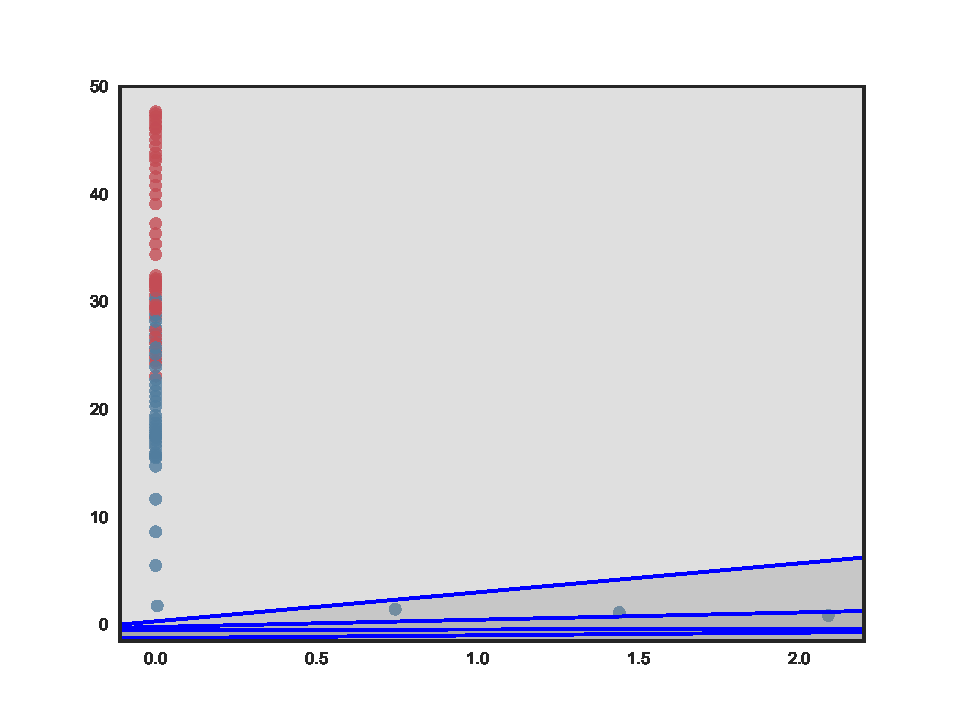
\includegraphics[width=\hsize]{img/toy/unitpointwise/conv2d_4-2.pdf}} 
    }
    % \hskip1em
    \parbox{.195\textwidth}{%
      \subcaptionbox{25th layer}{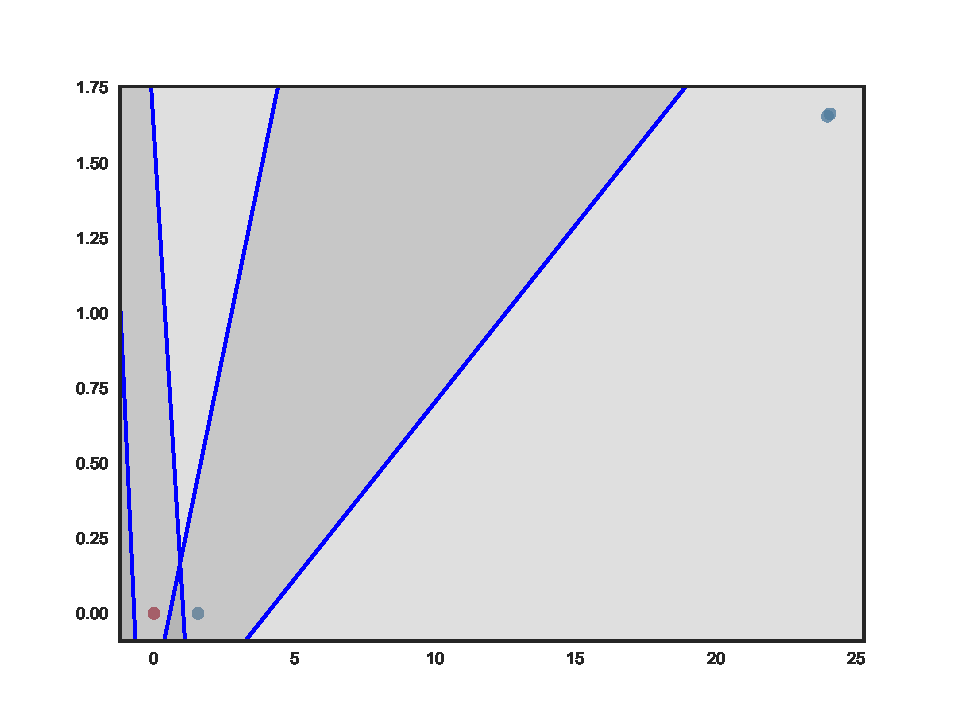
\includegraphics[width=\hsize]{img/toy/unitpointwise/conv2d_25-0.pdf}}
    %   \vskip1em
      \subcaptionbox{25th layer}{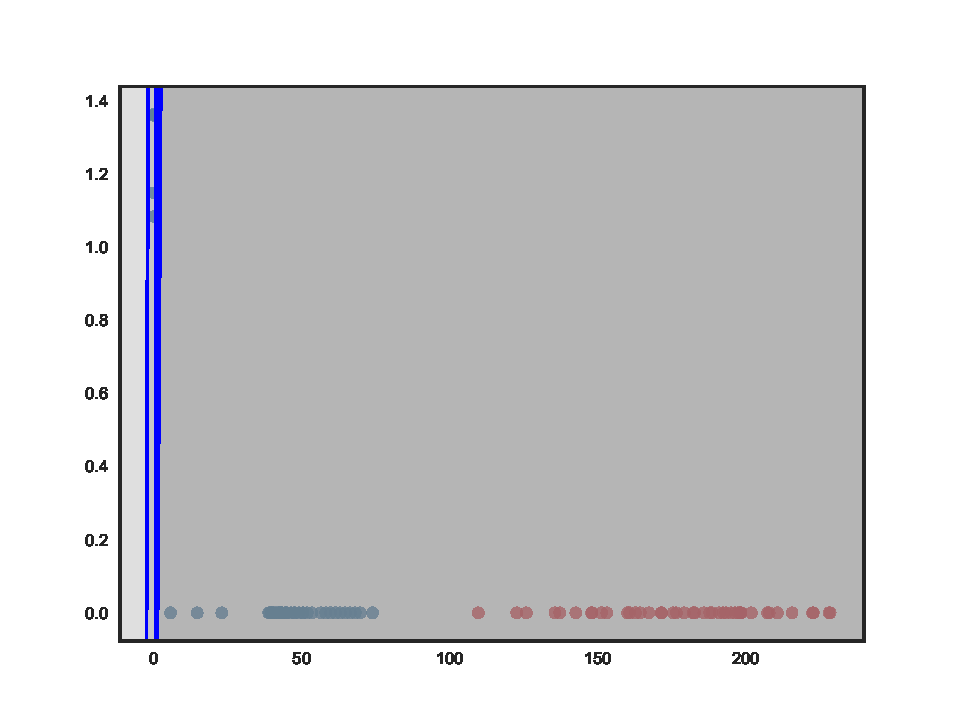
\includegraphics[width=\hsize]{img/toy/unitpointwise/conv2d_25-2.pdf}} 
    }
    % \hskip1em
    \parbox{.195\textwidth}{%
      \subcaptionbox{Feature layer}{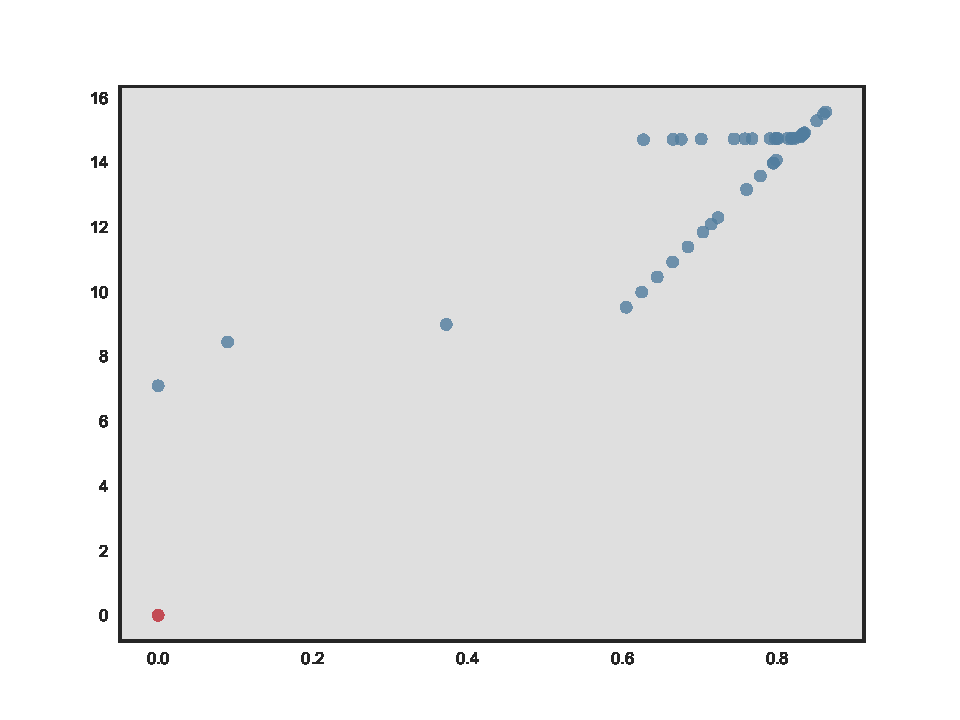
\includegraphics[width=\hsize]{img/toy/unitpointwise/dense_1-0.pdf}}
    %   \vskip1em
      \subcaptionbox{Feature layer}{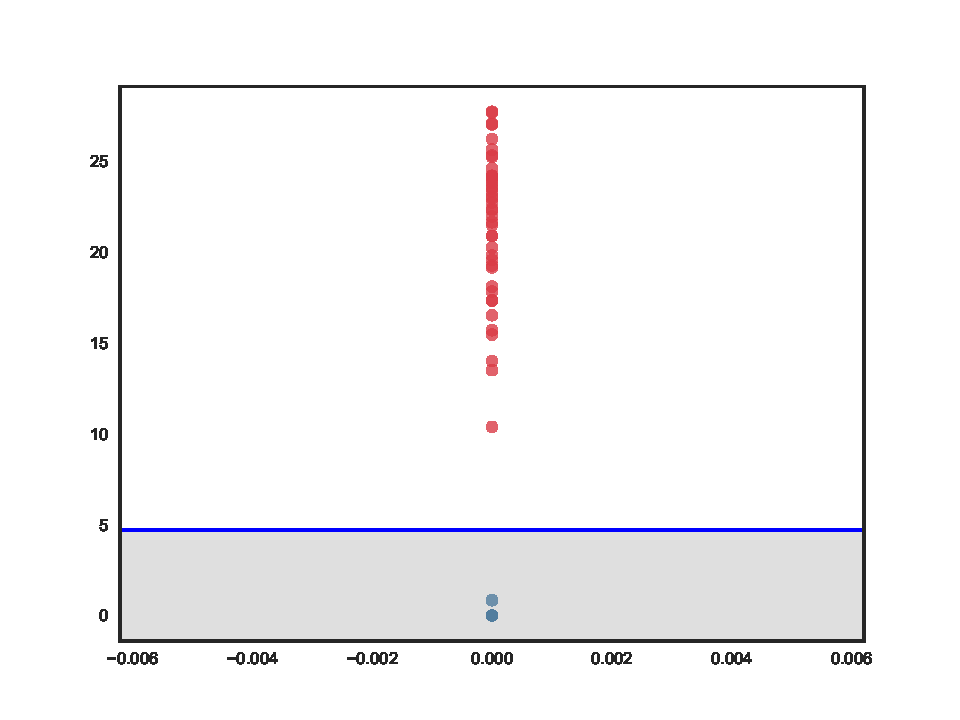
\includegraphics[width=\hsize]{img/toy/unitpointwise/dense_1-2.pdf}} 
    }
    % \hskip1em
    \parbox{.195\textwidth}{%
      \subcaptionbox{Output}{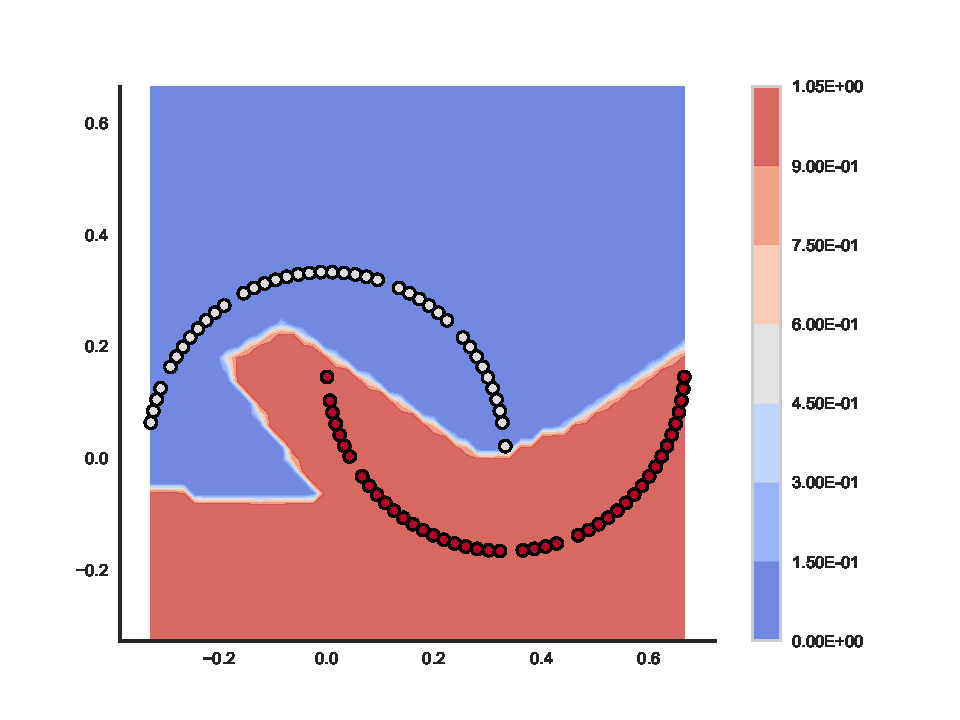
\includegraphics[width=\hsize]{img/toy/unitpointwise/output.pdf}}
    }
  }

    \caption{\SepUnitPoint}
    \label{fig:moonsUnitpointwise}
\end{figure*}

Finally, if we combine \SepPoint with \SepPoint in \SepUnitPoint, we find how is effectively separating the data at Figure \ref{fig:moonsUnitpointwise} (h). The solution found is a bit different from \SepLayer at Figure \ref{fig:moonsLayerwise}(h).

\subsection{The Effect of Constraint Loss}\label{subsec:effectConstraintLoss}

One interesting question is to understand which effect has the separation constraint by itself, without loss functional. Therefore, we train the same 50x4 network and hyperparameters than the experiment from \ref{subsec:classification}. Then we leave the network to optimize the different constraints that we propose to see what is the result of enforcing separation and nothing else. We use \ReLU and \ReLUBN for comparison purposes. 

We find that both \ReLU and \ReLUBN send concentrate all the data either in a single point in the case of \ReLU and two points in the case of \ReLUBN, see figure \ref{fig:init}. This explains the failure in \ref{fig:moonsReLU} and \ref{fig:moonsReLUBN}. In the other hand, we find how \SepLayer connects the output with in the input by sort of linearizing the network, thus outputting something very similar to a linear classifier. This is consistent with \cite{batchnormGradientExplosion}, where the authors prove that the network performs best as the units work closest to the linear regime. However, in their work they force \emph{tanh} activations into their linear regime to find that the depth is increased, whereas we leave the network to decide the units when is better to use a affine transform, to disable itself or perform in a non-linear manner. If we use \SepUnitPoint, we see that we lose smoothness but the feature representation is still reasonable, showing connectivity among the points, proof that up to some extent topological structure is preserved. Notice how the shape of the input layer is quite similar to the final solution found in Figure \ref{fig:moonsUnitpointwise}(a) when using a loss functional, but the feature layer is much richer. 

All of this translates into the dynamics shown in figure \ref{fig:peaks}, where we can see the convergence plot for \SepUnitPoint. The constraint loss pulls the weights into directions which harm cross-entropy, thus lowering accuracy, but that are better on the long run, so when cross-entropy converges the network achieves better accuracy than before the drop. Nevertheless, this behaviour is not always consistent and sometimes the constraint loss break the training process after some iterations, thus further research is required in this regard.

\begin{figure*}
  \centering
    \begin{subfigure}[b]{0.3\textwidth}
        \includegraphics[width=\textwidth]{img/init/relu/conv2d_1-0.pdf}
        \caption{\ReLU input layer}
        \label{fig:reluInitInput}
    \end{subfigure}
    ~ %add desired spacing between images, e. g. ~, \quad, \qquad, \hfill etc. 
      %(or a blank line to force the subfigure onto a new line)
    \begin{subfigure}[b]{0.3\textwidth}
        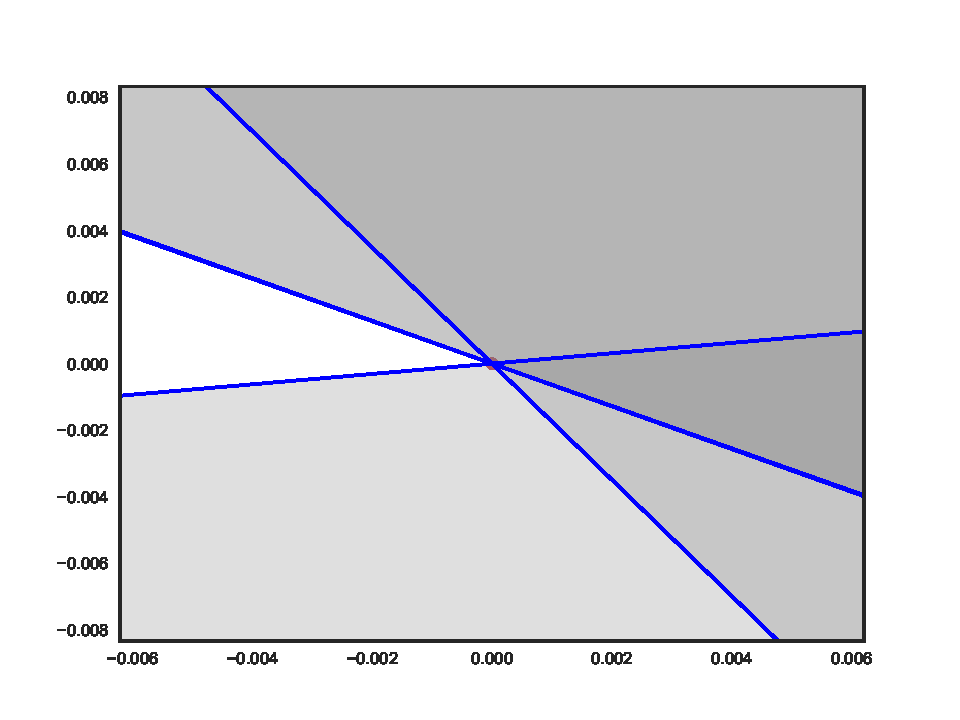
\includegraphics[width=\textwidth]{img/init/relu/conv2d_50-0.pdf}
        \caption{\ReLU 50th layer}
        \label{fig:reluInit501}
    \end{subfigure}
    ~ %add desired spacing between images, e. g. ~, \quad, \qquad, \hfill etc. 
    %(or a blank line to force the subfigure onto a new line)
    \begin{subfigure}[b]{0.3\textwidth}
        \includegraphics[width=\textwidth]{img/init/relu/conv2d_50-2.pdf}
        \caption{\ReLU 50th layer}
        \label{fig:reluIniti502}
    \end{subfigure}
    \\
    \begin{subfigure}[b]{0.3\textwidth}
        \includegraphics[width=\textwidth]{img/init/relu-bn/conv2d_1-0.pdf}
        \caption{\ReLUBN input layer}
        \label{fig:reluBNInitInput}
    \end{subfigure}
    ~ %add desired spacing between images, e. g. ~, \quad, \qquad, \hfill etc. 
      %(or a blank line to force the subfigure onto a new line)
    \begin{subfigure}[b]{0.3\textwidth}
        \includegraphics[width=\textwidth]{img/init/relu-bn/conv2d_50-0.pdf}
        \caption{\ReLUBN 50th layer}
        \label{fig:reluBNInit501}
    \end{subfigure}
    ~ %add desired spacing between images, e. g. ~, \quad, \qquad, \hfill etc. 
    %(or a blank line to force the subfigure onto a new line)
    \begin{subfigure}[b]{0.3\textwidth}
        \includegraphics[width=\textwidth]{img/init/relu-bn/conv2d_50-2.pdf}
        \caption{\ReLUBN 50th layer}
        \label{fig:reluBNInit502}
    \end{subfigure}
    \\
    \begin{subfigure}[b]{0.3\textwidth}
        \includegraphics[width=\textwidth]{img/init/layerwise/conv2d_1-0.pdf}
        \caption{\SepLayer input layer}
        \label{fig:layerwiseInitInput}
    \end{subfigure}
    ~ %add desired spacing between images, e. g. ~, \quad, \qquad, \hfill etc. 
      %(or a blank line to force the subfigure onto a new line)
    \begin{subfigure}[b]{0.3\textwidth}
        \includegraphics[width=\textwidth]{img/init/layerwise/conv2d_50-0.pdf}
        \caption{\SepLayer 50th layer}
        \label{fig:layerwiseInit501}
    \end{subfigure}
    ~ %add desired spacing between images, e. g. ~, \quad, \qquad, \hfill etc. 
    %(or a blank line to force the subfigure onto a new line)
    \begin{subfigure}[b]{0.3\textwidth}
        \includegraphics[width=\textwidth]{img/init/layerwise/conv2d_50-2.pdf}
        \caption{\SepLayer 50th layer}
        \label{fig:layerwiseInit502}
    \end{subfigure}
    \\
    \begin{subfigure}[b]{0.3\textwidth}
        \includegraphics[width=\textwidth]{img/init/unitpointwise/conv2d_1-0.pdf}
        \caption{\SepUnitPoint Input}
        \label{fig:unitpointInitInput}
    \end{subfigure}
    ~ %add desired spacing between images, e. g. ~, \quad, \qquad, \hfill etc. 
      %(or a blank line to force the subfigure onto a new line)
    \begin{subfigure}[b]{0.3\textwidth}
        \includegraphics[width=\textwidth]{img/init/unitpointwise/conv2d_50-0.pdf}
        \caption{\SepUnitPoint 50th layer}
        \label{fig:unitpointInit501}
    \end{subfigure}
    ~ %add desired spacing between images, e. g. ~, \quad, \qquad, \hfill etc. 
    %(or a blank line to force the subfigure onto a new line)
    \begin{subfigure}[b]{0.3\textwidth}
        \includegraphics[width=\textwidth]{img/init/unitpointwise/conv2d_50-2.pdf}
        \caption{\SepUnitPoint 50th layer}
        \label{fig:unitpointInit5012}
    \end{subfigure}
    
  \caption{} 
  \label{fig:init} 
\end{figure*}





\begin{figure*}[h]
  \begin{center}
    \includegraphics[width=1.0\textwidth]{peaks}
      \caption{Evolution of training throughout epochs (cross-entropy, constraint loss, and accuracy). Left-hand axis show the accuracy metric (blue line) against the cross-entropy, and constraint loss in the right axis (orange line), for each epoch of the training phase in the horizontal axis.}
			\label{fig:peaks}
\end{center}
\end{figure*}





\subsubsection{Zero initialization}\label{subsec:zero}

Since our constraint does not depend on the output of the layer but on its input, we can use it to initialize the parameters to zero and pull them from there. However, since all the units in the layer will share the same gradient and the constraints will be violated equally we need a way to fix those problems, which are the introduction of the balance between the positive and negative constraints, see \ref{eq:definitionOfRho}. Additionally, since all the weights of the same layer will receive the same gradient and will result in the same unit, we use Dropout \cite{dropout} in order to \emph{break symmetry}. We find that Dropout has a very strong effect harming convergence. This is why we choose to use annealing \cite{dropoutAnnealing}, starting with a high rate of 0.5 for 500 epochs with linear decay. See Figure \ref{fig:zeros} to see how the network evolves until finds a solution. We would like to remark that in this setup the training dynamics become particularly wild, with several peaks in the constraint loss which ultimately lead to the readjustement of the planes so a solution can be found. Also, we find this process highly depending on the planes found during the dropout process, introducing a new stochastic behaviour that we are not fond of. Better ways to fix this issue thus remain for future work.



\begin{figure*}
  \centering
    \begin{subfigure}[b]{0.3\textwidth}
        \includegraphics[width=\textwidth]{img/zero/1000/09-conv2d_1-0.pdf}
        \caption{1000 epochs}
        \label{fig:zerosInput1000}
    \end{subfigure}
    ~ %add desired spacing between images, e. g. ~, \quad, \qquad, \hfill etc. 
      %(or a blank line to force the subfigure onto a new line)
    \begin{subfigure}[b]{0.3\textwidth}
        \includegraphics[width=\textwidth]{img/zero/1000/57-09-output.pdf}
        \caption{1000 epochs}
        \label{fig:zerosOutput1000}
    \end{subfigure}
    \\
    \begin{subfigure}[b]{0.3\textwidth}
        \includegraphics[width=\textwidth]{img/zero/2000/09-conv2d_1-0.pdf}
        \caption{2000 epochs}
        \label{fig:zerosInput2000}
    \end{subfigure}
    ~ %add desired spacing between images, e. g. ~, \quad, \qquad, \hfill etc. 
      %(or a blank line to force the subfigure onto a new line)
    \begin{subfigure}[b]{0.3\textwidth}
        \includegraphics[width=\textwidth]{img/zero/2000/57-09-output.pdf}
        \caption{2000 epochs}
        \label{fig:zerosOutput2000}
    \end{subfigure}
    \\
    \begin{subfigure}[b]{0.3\textwidth}
        \includegraphics[width=\textwidth]{img/zero/3000/09-conv2d_1-0.pdf}
        \caption{3000 epochs}
        \label{fig:zerosInput3000}
    \end{subfigure}
    ~ %add desired spacing between images, e. g. ~, \quad, \qquad, \hfill etc. 
      %(or a blank line to force the subfigure onto a new line)
    \begin{subfigure}[b]{0.3\textwidth}
        \includegraphics[width=\textwidth]{img/zero/3000/57-09-output.pdf}
        \caption{3000 epochs}
        \label{fig:zerosOutput3000}
    \end{subfigure}
    
      
  \caption{.} 
  \label{fig:zeros} 
\end{figure*}


\subsection{Results concerning Accuracy}\label{subsec:accuracyResults}

To gauge accuracy between \ReLU, \ReLU +  batchnorm (\ReLUBN), and our proposal we tested all variants of our constraint using the same setup as \ref{subsec:classification}. We sampled $100$ points ($85$ for training and $15$). We used a 50x4 network. As hyper-parameters, we used learning rates $\gamma \in \{0.01, 0.001, 0.0001\}$, a batch size $bs = 85$, constraint loss parameter $\lambda = 0.01$ when needed, and set the number of epochs to $T = 2000$. We used the Glorot initialization scheme \cite{Glorot10Initialization}. 
 
We find how any of \SepConstraint versions show significant improvements over the \ReLU and \ReLUBN baselines (which yield \emph{trivial} validation accuracies of $40$\% and $60$\%, respectively). In the other hand, we see how \SepLayer achieves perfect accuracy closely followed by \SepUnitPoint, whereas \SepUnit and \SepPoint lag a bit behind, mirroring the results from \ref{subsec:classification}. The reader can observe Table \ref{tab:moons} for further detail.


\begin{table}[h!]
\begin{center}
\begin{tabular}{l|rr|rr}
\toprule
{}  & \multicolumn{2}{c}{Accuracy} & \multicolumn{2}{c}{Loss} \\
{}  & Train   & Val.  & Train  & Val.  \\
\midrule
\ReLU            &  0.5176 &      0.4 &  0.6925 &  0.6938 \\
\ReLUBN     &  0.8117 &      0.6 &  0.6331 &  0.6636 \\
\SepLayer &  1.0000 &      1.0 &  0.0000 &  0.0211 \\
\SepPoint    &  0.9294 &  0.8000 &  0.1765 &  0.6476 \\
\SepUnit    &  0.9058 &  0.8000 &  0.4161 &  1.5228 \\
\SepUnitPoint   &  0.9882 &  0.9333 &  0.6988 &  1.0810 \\
\bottomrule
\end{tabular}
\end{center}
\caption{Maximal performance experiment using the \moons dataset. From left to right, accuracy and loss (for \emph{train} and \emph{validation} sets) for \ReLU, \ReLUBN, and  \SepConstraint in all its variants.}
  \label{tab:moons}
\end{table}

